\documentclass[a4paper, 12pt]{report}
\usepackage{times}
\usepackage{graphicx}
\usepackage{latexsym}
\usepackage{morefloats}
\usepackage{color}
%\usepackage{enumitem}
\usepackage{verbatim}
\usepackage{xcolor,colortbl}
\usepackage{amssymb}
\usepackage{caption}
\usepackage{mathtools}
\usepackage{cleveref}
\usepackage{amssymb}
\usepackage{footnote}
\usepackage{graphicx}
\usepackage{indentfirst}
\usepackage{setspace}
\usepackage{graphicx}
\usepackage{caption}
\usepackage{capt-of}
\usepackage{multirow}
\usepackage{xcolor}
\usepackage{listings,xcolor}
\usepackage{float}
\usepackage{subcaption} 
\usepackage{algorithm}
\usepackage{algpseudocode} 
\usepackage{geometry}
\usepackage{hyperref}
\usepackage{kpfonts}
\usepackage{amsmath}
\usepackage{datetime}
\newdateformat{specialdate}{\twodigit{\THEDAY}-\twodigit{\THEMONTH}-\twodigit{\THEYEAR}}
\usepackage{nomencl}
\makenomenclature
\renewcommand{\nomname}{Summary of notation}
\nomenclature{$c$}{Speed of light} %ADD MORE NOTATIONS HERE
\hypersetup{colorlinks,linkcolor=black,citecolor=blue}

\linespread{1.1}

\newtheorem{definition} {Definition}

\geometry{a4paper,top=3cm,left=3cm,right=2.5cm,bottom=2cm}

\pagestyle{headings}
\begin{document}


% RO
 
 \begin{titlepage}
 
\sloppy
\begin{center}
\Large{UNIVERSITATEA BABE\c{S}-BOLYAI}\\
\vspace{0.2cm}
\Large{FACULTATEA DE MATEMATIC\u A \c SI INFORMATIC\u A}\\
\vspace{0.2cm}
\Large{SPECIALIZAREA INFORMATIC\u A}\\
\end{center}

\vspace{3.5 cm}
\begin{center}
\Huge \textbf{LUCRARE DE LICEN\c T\u A}\\
\vspace{1 cm}

\huge \textbf{Optimizarea transmiterii datelor \^ in patrularea cu re\c tele multi-robot}
\end{center}

\vspace{3.5cm}

\begin{flushleft}
\Large{\textbf{Coordonator \c stiin\c tific}}\\
\Large{\textbf{Prof. dr. Czibula Gabriela}}
\end{flushleft}

\vspace{2.5cm}

\begin{flushright}
\Large{\textbf{Student}}\\
\Large{\textbf{B\u adi\c t\u a Marin-Georgian}}
\end{flushright}

\vspace{1 cm}
\begin{center}
\Large{2020}
\end{center}

\end{titlepage}

%EN
\begin{titlepage}
\sloppy
\begin{center}
\Large{BABE\c{S}-BOLYAI UNIVERSITY}

\Large{FACULTY OF MATHEMATICS AND COMPUTER SCIENCE}
\end{center}
\vspace{3.5 cm}
\begin{center}
\Huge \textbf{DIPLOMA THESIS}\\
\vspace{1 cm}

\huge \textbf{Data Delivery Optimization in Multi-Robot Network Patrolling}
\end{center}

\vspace{3.5cm}

\begin{flushleft}
\Large{\textbf{Scientific supervisor}}\\
\Large{\textbf{Prof. dr. Czibula Gabriela}}
\end{flushleft}

\vspace{1.5cm}

\begin{flushright}
\Large{\textbf{Student}}\\
\Large{\textbf{B\u adi\c t\u a Marin-Georgian}}
\end{flushright}


\vspace{2cm}
\begin{center}
\Large{2020}
\end{center}

\end{titlepage}

\begin{abstract}
\par The subject of this thesis is the domain of Multi-Robot Patrolling (MRP). This thesis tackles a specific problem in the MRP called Data Delivery Optimization in Multi-Robot Network Patrolling. The MRP is a new research field with high potential for massive discoveries.
\par The thesis is structured in four chapters. In the first chapter some of the main concepts about multi-robot patrolling and reinforcement learning are introduced, while also reviewing the current literature about MRP. In the second chapter a novel approach to the Data Delivery Optimization problem, based the on a Dynamic Network Flows algorithm, is discussed, called \emph{DynFloR}. The following chapter aims to prove that a reinforcement learning approach to the problem is highly feasible, by introducing and testing a Q-learning model. The last chapter presents the software solution which solves the Data Delivery Optimization problem, providing details of the software development methodology used and implementation details.
\par The main elements of originality of this thesis consist in two new approaches to the problem, one based on Dynamic Network Flows (\emph{DynFloR}) and another one based on Reinforcement Learning (\emph{DronemRL}). A further original contribution consists in creating and designing the application showcased in the last chapter, as to the best of my knowledge there exists no application for creating, training and testing MRP environments publicly available.
\par This work is the result of my own activity. I have neither given nor received unauthorized assistance on this work.


\begin{flushright}

B\u{a}di\c{t}\u{a} Marin-Georgian
\end{flushright}

\begin{flushleft}
Cluj-Napoca\\
\specialdate\today
\end{flushleft}
\end{abstract}
 
    
\begin{comment}
%Pentru bursa
%
%+Pagina engleza
 \begin{titlepage}
 
\sloppy
\begin{center}
\Large{UNIVERSITATEA BABE\c{S}-BOLYAI}\\
\vspace{0.2cm}
\Large{FACULTATEA DE MATEMATIC\u A \c SI INFORMATIC\u A}\\
\vspace{0.2cm}
\Large{SPECIALIZAREA INFORMATIC\u A}\\
\end{center}

\vspace{2.5 cm}
\begin{center}
\Huge \textbf{RAPORT FINAL BURS\u A}\\
\vspace{1 cm}

\huge \textbf{Optimizarea transmiterii datelor \^ in patrularea cu re\c tele multi-robot folosind \^ inv\u a\c tare prin \^int\u arire}
\end{center}

\vspace{2.5cm}

\begin{flushleft}
\Large{\textbf{Coordonator \c stiin\c tific}}\\
\Large{\textbf{Prof. dr. Czibula Gabriela}}
\end{flushleft}

\vspace{0.5cm}

\begin{flushright}
\Large{\textbf{Student}}\\
\Large{\textbf{B\u adi\c t\u a Marin-Georgian}}
\end{flushright}

\vspace{1 cm}
\begin{center}
\Large{2019}
\end{center}

\end{titlepage}

\end{comment}

\setstretch{1.25}
\tableofcontents
\listoffigures
\listoftables
\listofalgorithms
\nopagebreak[0]


\chapter*{Introduction}
\addcontentsline{toc}{chapter}{\textbf{Introduction}}
\label{introduction}

\textbf{Patrolling} represents the repeated visit of certain places, over an area. The \emph{multi-robot patrolling} (also called \textit{multi-agent patrolling}) problem (MRP) consists in minimizing the time between two consecutive visits of the same place (called \emph{idleness}), using two or more robots. In the literature, this problem is generally considered to be NP-hard, while solutions often involve cyclic paths \cite{3,4}. Applications of the multi-agent patrolling problem include: surveillance tasks (e.g. anomaly detection, intruder detection), area coverage, data collection tasks (e.g. for the case of wireless sensor networks - WSNs), rescue operations (e.g. people or objects in dangerous situations) \cite{1,2}. 


A major challenge when deploying fleets of mobile robots in real scenarios/environments is  the ability of the robots to adapt to the complexity of their environment, that is its dynamics and uncertainty. In such dynamic environments the robots need to be able to provide robust solutions to complex tasks and to adapt to changes in their environment. The multi-agent patrolling task is intensively investigated within the multi-agent research community and various algorithms based on reactive and cognitive architectures have been introduced \cite{othmaniguibourg18}.

This thesis offers solutions for optimizing data delivery in multi-robot network patrolling in the scenario where the environment is deterministic, the network of robots is centralized and offline and the robots have periodic meetings and also aims to prove that in a more general scenario of the multi-robot network patrolling, where the patrolling environment is non-deterministic and uncertain a \emph{reinforcement learning} approach is feasible. The problem was proposed in a bilateral collaboration between the MLYRE team from Cluj-Napoca coordinated by prof. Gabriela Czibula and the CHROMA team from Insa Lyon coordinated by prof. Olivier Simonin.

\par The rest of the thesis is structured as follows. Chapter \ref{bck} presents the background concepts used in this thesis, while our Dynamic Network Flows algorithm is outlined in Chapter \ref{flow}. Chapter \ref{rl} is concerned with proving that a \emph{reinforcement learning} approach is feasible and a detailed software solution is presented in  Chapter \ref{softwareApplication}. \\
The conclusions of our thesis and directions to further continue and improve our research are given in Section \ref{conclus}.


\chapter*{List of publications}
\addcontentsline{toc}{chapter}{\textbf{List of publications}}

\begin{normalsize}

\begin{enumerate}

\item [\cite{kes}] Vlad-Sebastian Ionescu, Zsuzsanna One\c t-Marian, \textbf{Marin-Georgian B\u adi\c t\u a}, Gabriela Czibula, Mihai-Ioan Popescu, Jilles S. Dibangoye, Olivier Simonin.
\newblock {$\mathit{DynFloR}$: \emph{A Flow Approach for Data Delivery Optimization in Multi-Robot Network Patrolling}}.
\newblock 23rd International Conference on Knowledge-Based and Intelligent Information \& Engineering Systems (KES 2019), Procedia Computer Science  Vol 159, (2019)  pp. 97-106 (\textbf{ISI Proceedings}). 

\end{enumerate}

\end{normalsize}


\chapter{Background}\label{bck}


The MRP is a relatively new field in research, with high potential for discoveries, but yet at the same time with its own challenges, mostly concerning uncertain and dynamic environments.
\par The purpose of this chapter  introduce some of the main concepts used in this thesis, by creating an underlying basis for the patrolling problem and its place in the research world. The chapter is structured as follows. The Multi-robot patrolling problem is explained and detailed in Section 1.1. A general introduction to Reinforcement Learning is presented in Section 1.2, while Section 1.3 contains a literature review on the \emph{multi-robot} network patrolling.

\section{Multi-robot patrolling}

\textbf{Patrolling} represents the repeated visit of certain places, over an area. The \emph{multi-robot patrolling} (also called \textit{multi-agent patrolling}) problem (MRP) consists in minimizing the time between two consecutive visits of the same place (called \emph{idleness}), using two or more robots. In the literature, this problem is generally considered to be NP-hard, while solutions often involve cyclic paths \cite{3,4}. Applications of the multi-agent patrolling problem include: surveillance tasks (e.g. anomaly detection, intruder detection), area coverage, data collection tasks (e.g. for the case of wireless sensor networks - WSNs), rescue operations (e.g. people or objects in dangerous situations) \cite{1,2}.  Figure \ref{patrolling} illustrates a solution for the case of data collection in WSNs (from \cite{8}).

\begin{comment}
\begin{figure}[htb]
\centering
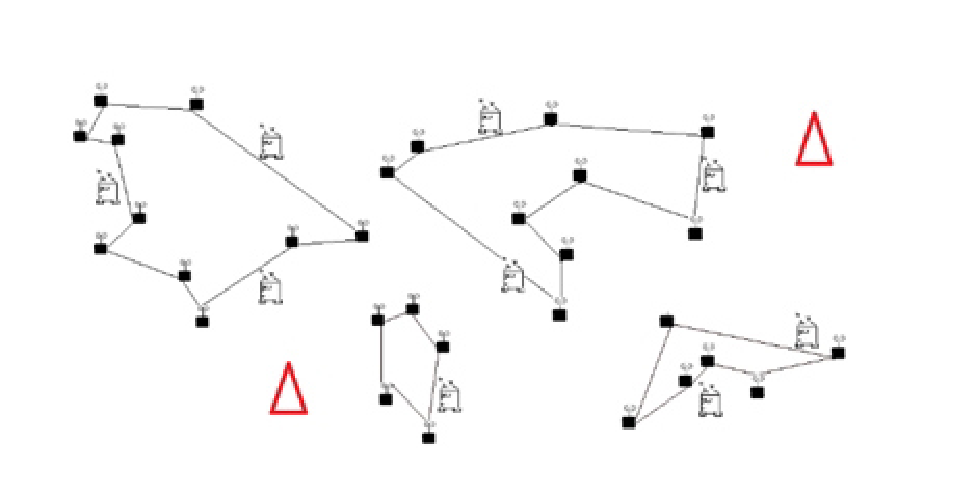
\includegraphics[scale=0.5]{Figures/Patrolling.pdf}
\caption{An example of multi-robot network patrolling \cite{8}.}
\label{patrolling}
\end{figure}
\end{comment}


We consider the general case of the patrolling of specific places with a fleet of robots.  \emph{Multi-robot patrolling} consists in organizing the continuous coverage of an area by several agents, e.g. drones, autonomous vehicles etc. The problem of \emph{multi-robot patrolling} with minimum visiting frequency has been formalized in \cite{8} as a \emph{clustering} problem. Considering that $T=\{t_1, t_2,\cdots, t_n\}$ is a set of targets that have to be patrolled, a patrolling solution may be viewed as a partition $\mathcal{K}=\{K_1, K_2, \cdots, K_p\}$ of $T$ ($K_i \subseteq T, K_i \neq \emptyset, \forall 1 \leq i \leq p$ and $T =\displaystyle\bigcup_{i=1}^{p} K_i$ and  $K_i \cap K_j =\emptyset, \ \forall 1 \leq i, j \leq p, i \neq j $) with minimum $p$. In addition, $length(C_i) \leq B$, where $C_i$ is the cycle formed on cluster $K_i, 1\leq i \leq p$, and $B$ is a given bound imposed on the cycles' length,  required  due  to  the  minimum  visiting  frequency that has to be achieved in the target patrolling.


A major challenge when deploying fleets of mobile robots in real scenarios/environments is  the ability of the robots to adapt to the complexity of their environment, that is its dynamics and uncertainty. In such dynamic environments the robots need to be able to provide robust solutions to complex tasks and to adapt to changes in their environment. The multi-agent patrolling task is intensively investigated within the multi-agent research community and various algorithms based on reactive and cognitive architectures have been introduced \cite{othmaniguibourg18}. Still, the existing patrolling approaches are specific ones and those regarding dynamic environments  (\emph{dynamic multi-robot patrolling} - DMRP) are in early phases \cite{othmaniguibourg18}.  
An extended and more complex version of the patrolling is the \emph{dynamic patrolling}, in which places (or targets) to patrol will be discovered progressively by agents/robots that spread out in the environment. A challenge in such a setting  is to ensure that robots remain connected, i.e. are able to communicate, in order to cooperate and to pass collected data up to their base station (where they start). 

Starting from the formalization introduced in \cite{8}, the DMRP problem may be formalized as a \emph{dynamic clustering} problem. In the DMRP, two types of information are discovered online by the robots, and they are  required to adapt their current patrolling solution. First, the targets to patrol are not known a priori, they will be discovered while robots spread out in the environment. As the robots have to start to patrol as soon as they have detected some targets, they must modify their patrol when they discover new ones. The problem of adapting the clusters (cycles) when new targets are discovered has been approached by Popescu et al. \cite{dmap2018}, where a dynamic saturation-based auctioning algorithm (DSAT) was introduced  for a continuous adaptation of the multi-robot target allocation process (MRTA) to new discovered targets.

While the robots patrol a group (or a cluster) of targets by following a cyclic path and collect data from the targets, they have to pass collected data to their neighboring robots/cycles in order to communicate information to the base station. In network patrolling, each robot can have the choice to transmit collected data to different neighbors, i.e. to other close paths (cycles). 

\section{Reinforcement learning (RL)}

Since the beginning of computing, mathematicians and computer scientists were concerned about how to create programs or machines capable of learning in the same way as humans do, that is learning from interaction with our environment, which is a foundational idea underlying nearly all theories of learning and intelligence \cite{rsab} .
 \par Reinforcement learning (RL) deals with the problem of how an autonomous agent which is situated in an environment, perceives and acts upon it and also can learn to select optimal actions to achieve its goals \cite{mitchell}. Reinforcement learning is used in many practical problems, such as learning to control autonomous robots \cite{konidaris}, learning to find the solution of an optimization problem (such as operations in factories) or learning to play board games. In all these problems, the agent has to learn how to choose optimal actions in order to achieve its goals, through the reinforcements received after the interaction with its environment. 

In a reinforcement learning task, the learner tries to perform actions in the environment and it receives \emph{rewards} (or \emph{reinforcements}) in the form of numerical values that represent an evaluation of how good were the selected actions \cite{uribe}. The learner (agent) simply has a given goal to achieve and it must learn how to achieve that goal by trial-and-error interactions with the environment. RL is learning  how to map situations to actions in order to maximize the cumulative reward received when starting from some initial state and proceeding to a final state.  

A general RL task is characterized by four components \cite{rsab}. The \emph{environment} \emph{state space} $\mathcal{S}$  represents all possible states of an agent in the \emph{environment}, for example every cell on a word represented as a grid. The \emph{action space} $\mathcal{A}$ consists of all  actions that the learning agent can perform in the environment. The \emph{transition function} $\delta$ specifies the non-deterministic behavior of the environment (i.e. the possibly stochastic outcomes of taking each action in any state). The last component of the RL task is the \emph{reinforcement (reward)  function} which defines the possible reward of taking an action in a particular state.

The agent's task in a reinforcement learning scenario is to learn an \emph{optimal policy}, $\pi: \mathcal{S} \rightarrow \mathcal{A}$, that maximizes the expected sum of the delayed rewards for all states $s$: $$V^{\pi}(s)=\sum_{i=0}^{n} r_i \cdot \gamma^i$$ The future rewards are discounted exponentially by their delay and $\gamma$ ($0 \leq \gamma <1$)  is the discount factor for the future rewards.

\subsection{Q-learning}\label{qLearningAlgo}

A popular and effective RL method is considered to be the \emph{Q-learning} algorithm \cite{rsab}. In this scenario, the agent learns an \emph{action-value function} (\emph{Q}) giving the expected utility of taking a given action in a given state.  In such a scenario, the agent does not need to have a model of its environment.

For training the RL agent, a $Q$-learning approach is usually used, in which the agent learns the $Q$-value function that gives the expected utility of performing an action in a given state \cite{rsab}. The training process consist of the following. Through a number of training episodes, the agent will try (possible optimal) \emph{candidate solution} paths from the initial to a final state. After performing an action in its environment, the agent will receive rewards and will update the $Q$-values estimations according to the \emph{Bellman's equation} \cite{dayan} where $Q(s,a)$ denotes the estimation of the \emph{Q-value} associated to the state $s$ and action $a$, $\alpha$ represents the learning rate and $\gamma$ is the discount factor for future rewards.
$$ \text{Bellman's equation: } Q(s,a) = Q(s,a) + \alpha\cdot(r + \gamma \cdot \max_{a' \in A}Q(s', a')-Q(s,a))$$
The general form of the $Q-Learning$ algorithm is given in Algorithm 1:

{} \hrulefill {}

\begin{footnotesize}

\hspace{0cm}Repeat

\hspace{0.25cm}Select the initial state of the agent in the environment as $s_1$.

\hspace{0.25cm}Select action $a$ from $s$ using an action selection mechanism.

\hspace{0.25cm}Repeat

\hspace{0.5cm}Perform action $a$, observe the reward $r$ and the next state of the environment $s'$.

\hspace{0.5cm}Update the value $Q(s,a)$ as follows

$$Q(s,a)=Q(s,a)+\alpha \cdot (r+\gamma \cdot \max_{a' \in \mathcal{A}} Q(s',a')-Q(s,a))$$

\hspace{0.5cm}s $\leftarrow$ s'

\hspace{0.25cm}until $s$ is terminal

\hspace{0cm}Until the maximum number of episodes is reached or the $Q$-values do not change

\end{footnotesize}

{} \hrulefill {} 	  		

\begin{center}
\textbf{Algorithm 1. The Q-learning algorithm \cite{watkins}.}
\end{center}

\newpage
\section{Literature review on \emph{multi-robot} network patrolling}\label{lr}

The field of the multi-robot patrolling is relatively recent, with various contributions which are mainly based on operational research. The networks are usually represented as graphs, where the nodes are critical points (targets) that should be visited as often as possible and the edges represent paths between these  targets. 

Graph based algorithms were used for various patrolling tasks: Hamiltonian cycles for assuring that each point in the target area is covered at the same optimal frequency \cite{Elmaliach:2009}, cyclic strategies which use heuristics to compute TSP cycles \cite{Chevaleyre2004}, path-finding techniques for implementing the decision making strategy for the agents. %\cite{Machado_2002}. 
Alternative approaches in multi-robot patrolling use classical techniques for computational agents coordination in certain environments \cite{portugal_2011},  cooperative auction systems \cite{Hwang_2009} and algorithms based on swarm intelligence \cite{chu_2007}. Santana et al. modelled the patrolling problem as a reinforcement learning problem \cite{Santana:2004}, for allowing the agents to automatically adapt to their environment with the goal of optimizing (maximizing or minimizing) a certain performance criterion (e.g. minimizing the nodes idleness). The authors have shown that the adaptive solutions are superior to other solutions mainly due to the work is distribution (no centralized communication) and the adaptive behavior of the agents, which can be desirable in this domain \cite{Santana:2004}.

Liemhetcharat et al. \cite{Liemhetcharat2015} approached the problem of foraging and item delivery with multi-robot networks. The authors proposed a formal model for the multi-robot item delivery problem and showed that the continuous foraging problem is a particular case of it. Distributed multi-robot algorithms were also proposed to solve the item delivery and foraging problems and experimented on simulated robots using a Java simulator. Chen et al.  \cite{Chen_2015} investigated  a multi-agent patrolling problem in uncertain environments. For dealing with uncertainty and possible threats, the environment was modelled as multi-state Markov chains, whose states are partially observable until the location is visited by an agent. The main goal of the approach from  \cite{Chen_2015} was to maximize the amount of information gathered by the agents while reducing the damage incurred.  Farinelli et al.  \cite{11} formalized the problem of coordination (i.e. establishing collaborative interactions between robots to achieve individual and collective goals) as a Distributed Constrained Optimization problem, providing a solution based on the binary max-sum algorithm. The problem of \emph{dynamic multi-robot patrolling} was recently approached by Othmani-Guibourg et al. \cite{othmaniguibourg18}. The authors proposed a formal model for dynamic environment and on edge-markovian evolving graphs and they introduced and analyzed two strategies for the agents for patrolling in dynamic environments. 





%\include{bursa}

\chapter[A Flow Approach for Data Delivery Optimization]{$\mathit{DynFloR}$: A Flow Approach for Data Delivery Optimization in Multi-Robot Network Patrolling}
\label{flow}

Deploying fleets of mobile robots in real scenarios and environments raises several scientific challenges. One of them concerns the ability of the robots to adapt to the dynamics of their environment. We introduce $\mathit{DynFloR}$ \cite{kes}, a dynamic network flow based approach for finding optimal policies for \emph{data delivery} in \emph{multi-robot network patrolling} where the robots can communicate instantly and free of charge one to another, there is a periodicity of the robot meetings and the distribution of the data collected during the patrol is regular. Experiments on randomly generated synthetic examples are performed for evaluating the performance of the $\mathit{DynFloR}$ method. The performed experiments empirically show that independent of the problem setting (such as number of robots, memory of the robots) the amount of data transferred to a base station per unit of time converges to an equilibrium state. The case of lost data has been also examined through various experiments, but it requires further experimentation as well as in-depth analysis. This chapter represents the first step in a research which is being conducted for using \emph{reinforcement learning} in order to optimize data delivery in a general multi-robot network patrolling case, when the patrolling environment is non-deterministic and uncertain.

The study performed  in this chapter represents the starting point of a broader research which is being conducted for optimizing data delivery in DMRP using \emph{reinforcement learning} (RL) \cite{AsisHHS18}, in the more general case when there is an uncertainty in the environment (i.e. there is no periodicity in the robots' meetings). In this general case, the robots will have to learn through \emph{reinforcement} (RL) \cite{Konidaris12} the data transfer policy, in order to maximize the quantity of transmitted data.
 
The contribution of this chapter consists in a new approach, $DynFloR$, based on dynamic network flows for determining the optimal policy for delivering data in multi-robot network patrolling under the following assumptions: the environment is deterministic, the network of robots is centralized and offline and the robots have periodic meetings. The proposed $DynFloR$ method adapts the approach proposed by  Kotnyek \cite{flow} for the problem of MRP. It can be also extended for the DMRP under the previously mentioned assumptions. We assume the data transfer to be dynamic and we address the following research question: \emph{How to optimize data-passing between each robot cycle in order to maximize the quantity of data transmitted to the sink?} Experiments and simulations performed on several synthetic and randomly generated examples emphasize that our proposal is able to determine a policy that maximizes the data transferred to the base station up to a given moment in time.  The answer to the previously stated RQ through the $DynFloR$ approach will provide us additional insights on the nondeterministic MRP/DMRP problem and its modelling as a reinforcement learning task. To the best of our knowledge, $DynFloR$ approach is new in the MRP literature.

The rest of the chapter is structured as follows.  Our $DynFloR$ approach for data delivery optimization in a deterministic setting of the MRP is introduced in Section \ref{our}. Section \ref{discussion} presents the experimental results obtained by evaluating $DynFloR$ and provides a comparison to existing similar approaches. Furthermore, in Section \ref{discussion} we have a discussion about the current solution as well as its advantages and limitations. Section \ref{conc} contains the conclusions of the chapter and directions to continue our research.

\section{Methodology}\label{our}

This section introduces our centralized and offline $DynFloR$ approach for data delivery optimization in a deterministic setting of the MRP. $DynFloR$ is  applicable in a deterministic setting of DMRP, as well. 

\subsection{Problem definition. Theoretical model}\label{tm}

The problem we are approaching in this chapter is defined in the following. We assume the particular case of a deterministic environment, in which the network of robots is centralized and offline:  \emph{There are $n$ robots, which can meet and exchange data. The robots are continuously collecting data on the cycles they patrol. There are initial meeting times for the robots and meeting periods. The goal is to maximize the quantity of data arriving to a sink (a base station) in a given time T}.

Let us consider the following theoretical model.  We denote by $\mathcal{R}=\{R_1, R_2, \cdots, R_n\}$ the set of patrolling robots. We assume the sink is denoted by $R_0$. Each robot $R_i \in \mathcal{R}$ patrols a certain cycle $C_i$ consisting of $k_i$ targets, i.e. $C_i=\{t_i^{1}, t_i^{2}, \dots t_i^{k_i}\}$. At each visit of the target $t_i^{j}$, an amount $d_i^{j}$ of data  will be collected by robot $R_i$. Hence, after patrolling a complete cycle, robot $R_i$ collects a quantity of data  $D_i=\displaystyle \sum_{j=1}^{k_i}{d_i^{j}}$. This data is stored in robot $R_i$'s memory, of maximum capacity $\mathit{MaxCapacity_i}$.  We consider that the sink has no memory limit, i.e. $MaxCapacity_0=\infty$. For data exchange, two robots $R_i$ and $R_j$ have periodical meetings (\emph{rendez-vous} points) starting at time  $T_{ij}$ when they first meet, with a period of $\pi_{ij}$ time steps.   

In our approach, we assume that the incoming data model is \emph{regular} and \emph{known} and that there is a single base station (called {\em sink}). The data is continuously collected by the robots after patrolling their cycle and has to be transmitted to the sink. We also assume that it takes one unit of time for a robot to go from one target to the next one and that transferring data does not take time.

Figure \ref{ex} depicts a synthetically generated example, a much simplified version of the MRP problem with 4 robots and 6 targets, in which data is static (i.e. collected only once by a robot, at the beginning of the simulation), the robots' meetings are periodical and the solution is the minimum time required for transferring all collected data to the \emph{sink} (denoted by R0). In Figure \ref{ex} $RV$ represents the meetings between the robots, $T_{ij}$ is the time stamp when robots $i$ and $j$ first meet and $\pi_{ij}$ is the meeting period for robots $i$ and $j$. Assuming that the initial data for every robot is $10$ and the maximum memory for all robots is $15$, the minimum time in which all data can be transferred to the sink is $8$. The right side table from Figure \ref{ex} depicts the decision making strategy for the agents, at each time moment, obtained using a brute force approach. Each line from the table represent a time moment and the columns from the second to the fifth indicate the target visited by the robots (including the sink) at a given time.  If two robots visit the same target at a given time, there is a meeting between them and data can be transferred. The last three columns on a row (time) present the data transfer strategy between the robots at that moment, i.e. robot \textbf{From} transfers to robot \textbf{To} the quantity \textbf{Quant}. 

\begin{figure}[!htb]
\centering
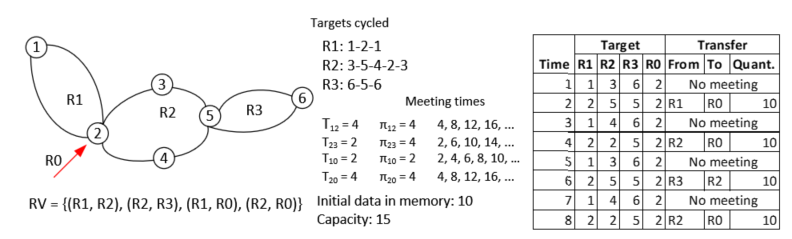
\includegraphics[scale=0.45]{Figures/KES_Figure3.png}
\caption{Synthetic example.}
\label{ex}
\end{figure}

\subsection{The proposed \emph{DynFloR} approach}\label{df}

For modeling the dynamic data collection process from the multi-robot network previously defined in Section \ref{tm}, we introduce a dynamic flow network based model which captures both the temporality of the patrolling process, as well as the dynamicity of the data collection and transfer. 

\subsubsection{The proposed dynamic network model}\label{model} 

Our proposed model adapts the dynamic network flow approach introduced in \cite{flow} by taking into account the specific requirements of multi-robot network patrolling. The flow network graph $G$ is constructed from moment 0 up to a moment of time $Time$. For each time step, the graph captures the state of each robot and the sink. Each of the states is represented by a node in the graph, which includes information such as robot decisions (data currently collected, data currently transferred, robot met for data exchange) or the amount of data stored. 

There are $(n+1) \cdot (Time+1) + 1$ \textbf{nodes} in the dynamic flow graph. For each robot $R_i$ including the sink ($\forall i, \; 0 \leq i \leq n$) there are $Time$+$1$ nodes, denoted by $i_t$ ($\forall t, \; 0 \leq t \leq Time$). The node $i_t$ corresponds to robot $R_i$ at time $t$. The \emph{sink} is viewed, in the proposed model, as robot $R_0$.  Besides the nodes corresponding to the robots, there is an additional \emph{source} node $s$ connected to all robots (except the sink) at time step 0.

The directed \textbf{edges} (connections) between the flow network's nodes and their capacities are set as follows. There is a connection between the source node $s$ and node $i_0$ ($\forall i, \;1 \leq i \leq n$) and its capacity is set to the the initial data $Q_i$ held by the robot $R_i$ at the beginning of the simulation. For each time moment $t$ when two robots $R_i$ and $R_j$ meet, two edges are added: one from $i_t$ to $j_t$ with capacity $\mathit{MaxCapacity_j}$ (i.e., the maximum memory of $R_j$) and one from $j_t$ to $i_t$ with capacity $\mathit{MaxCapacity_i}$ (i.e., the maximum memory of $R_i$). For each robot $R_i$ (including the sink) an edge is created between $i_t$ and $i_{t+1}$, $\forall t,\; 0 \leq t \leq Time-1$ (the edge has the capacity $\mathit{MaxCapacity_i}$). For each time moment $t$ when new data is collected by a robot $R_i$, an edge connecting the source node $s$ and the node $i_t$ is added and its capacity is set to $D_i$.      

We mention that the currently proposed model contains nodes corresponding to an entire cycle patrolled by a robot (without detailing the targets patrolled during each cycle). We also assume that a robot collects the data after it patrolled an entire cycle, this is why we add one edge with capacity $D_i$ after $k_i$ time units, instead of adding one edge with capacity $d_i$ to every node. The previous assumptions do not reduce the generality of $DynFloR$, as we can easily extend the model by adding new data at every time step to every robot and the $DynFloR$ algorithm remains the same. In this case, new data will be collected by a robot in a node corresponding to a target and not to an entire cycle (as in the current model).  

\subsubsection{$DynFloR$ algorithm}\label{dynflor}

After the flow network graph $G$ is built as described in Section \ref{model}, a maximum flow \cite{flow} from the source $s$ to the network sink (a node $0_t, t\leq Time$) will give the total amount of data that can be transferred to the base station in $t$ time steps.
Our proposal $\mathit{DynFloR}$ outputs the decision making strategy for each robot $R_i$, at each rendez-vous time, in order to increase the quantity of data received by the sink while respecting the memory constraint for each robot. 

The pseudocode for constructing the flow graph $G$ is presented in Algorithm \ref{alg:graph} and the $DynFloR$ algorithm is given in Algorithm \ref{alg:dynflor}. For determining the maximum flow in a graph $G$, the Preflow-Push algorithm \cite{Preflow} denoted by $getFlow$($G$) is used.  We also denoted by $addNode$ and $addEdge$ the operations for creating a node and an edge with a certain capacity, respectively. 

\begin{algorithm}[!htb]
\caption{Algorithm $DynFloR$}
    \label{alg:dynflor}
\begin{algorithmic}
\State{\textbf{Algorithm} $DynFloR$ is:}
\State{// determines the optimal policy for the robots' data delivery}
\Require{$n, k$ {\rmfamily - the number of robots and a list containing the robots' cycle lengths}
\\ \ \ \ {$D, Q, MaxCapacity$ \rmfamily - lists containing the amount of data collected by each robot, its initial data and its maximum memory}
\\ \ \ \ {$RV, Time$ \rmfamily - the list containing the pairs of robots that meet and the final moment of time considered}
\\ \ \ \ {$T, \pi$ \rmfamily - the initial meeting time for each pair of robots from $RV$ and their meeting period}
}
\Ensure{{\rmfamily returns the data delivery strategy for the robots from $RV$ (the path that gives the maximum flow in $G$)}}
\State{// read the input data}
\State{// construct the flow network graph $G$}
\State{$G \leftarrow CreateGraph$($n$,$k$,$D$,$Q$, $MaxCapacity$,$RV$,$Time$,$T$,$\pi$)}
\State{// the data delivery policy $Policy$ is computed from the path that corresponds to the maximum flow $MaxFlow$ in the graph $G$}
\State{$(MaxFlow, Policy) \leftarrow getFlow$($G$)}
\State{\textbf{EndAlgorithm} }
\end{algorithmic}
\end{algorithm}


\begin{algorithm}[!htb]
\caption{Function $CreateGraph$}
    \label{alg:graph}
\begin{algorithmic}
\Function{$CreateGraph$}{$n, k, D, Q, MaxCapacity,RV,Time,T,\pi$}
\State{// Create the flow network graph corresponding to the MRP problem}
\Require{$n, k, D, Q, MaxCapacity,RV,Time,T,\pi$ {\rmfamily the input parameters for the $DynFloR$ algorithm}}
\Ensure{returns the graph $G$ constructed as described in Section \ref{model}}
\State{// Create the nodes, edges and their capacities}
\State{$addNode$($G$,$s$) // a node corresponding to the source}
\For{$i \gets 0, n$}
\For{$t \gets 0, Time$}
\State{$addNode$($G$,$i_t$) // a node corresponding to robot $R_i$ at time $t$}
\If{$t \neq 0$}
\If{$i=0$}
\State{$addEdge$($G$,$i_{t-1}$,$i_t$,$\infty$)  // add an edge between $0_{t-1}$ and $0_t$ with capacity $\infty$}
\Else
%\State{// add an edge between $i_{t-1}$ and $i_t$ with capacity the memory of $R_i$}
\State{$addEdge$($G$,$i_{t-1}$,$i_t$,$MaxCapacity_i$) }
\EndIf
\EndIf
\EndFor
\If{$i \neq 0$} 
\State{$addEdge$($G$,$s$,$i_0$,$Q_i$)}% // add an edge between the source and $i_0$ with the  capacity of $D_i$}
\EndIf
\EndFor
\For{each pair $(i,j) \in RV$}
\For{$t \leftarrow T_{ij}, Time, \pi_{ij}$}
%\State{// add an edge corresponding to a possible transfer between $R_i$ and $R_j$ at time $t$}
\State{$addEdge$($G$,$i_t$,$j_t$,$MaxCapacity_i$)}
\If{$j \neq 0\;\;\;$} //if $j$ is not the sink 
%\State{// add an edge corresponding to a possible transfer between $R_j$ and $R_i$ at time $t$}
\State{$addEdge$($G$,$j_t$,$i_t$,$MaxCapacity_j$)} 
\EndIf
\EndFor
\EndFor
\State{// Add additional edges to model the data dynamically collected by the robots}
\For{$i \leftarrow 1, n$}
\For{$t \leftarrow 1, Time$}
\If{$t \;mod\; k_i=0\;\;$ // if an entire cycle was patrolled by robot $R_i$}
\State{// add an edge from the source to $i_t$ for modelling that new amount of data  $D_i$ arrives in the node}
\State{$addEdge$($G$,$s$,$i_t$,$D_i$)}
\EndIf
\EndFor
\EndFor
\State{// Return the graph $G$ }
\State{return $G$}
\EndFunction
\end{algorithmic}
\end{algorithm}

\noindent We note that the \emph{objective function} which has to be maximized in our approach is $$f(T)=\frac{data\;\;to\;\;sink\;\;until\;\;time\;\;T}{T}$$
Alternatively, we envisage the minimization of $$g(T) = \frac{input\;\; data\;\;-\;\;data\;\;to\;\;sink\;\;until\;\;time\;\;T}{T}$$

A brief analysis of the time complexity of $DynFloR$ is given below.  The time complexity of the $CreateGraph$ subalgorithm for constructing the dynamic network $G$ is $\mathcal{O}(|RV|\cdot Time)$. Therefore, the overall complexity of $DynFloR$, including computing the maximum flow, is $\mathcal{O}  \left( \mathcal{F}(n \cdot Time, |RV| \cdot Time) \right )$, where $\mathcal{F}(V, E)$ is the time complexity of a flow algorithm applied on a graph with $V$ nodes and $E$ edges (in our graph we have $n \cdot Time$ nodes and $|RV|\cdot Time$ directed edges). For example, for the highest label preflow-push algorithm \cite{Cormen:2009}, we have $\mathcal{F}=\mathcal{O} \left({(n \cdot Time)}^2 \cdot \sqrt{|RV|\cdot Time} \right)$. 



\subsection{Example}

For exemplifying how $DynFloR$ works, let us consider a very simple example of MRP illustrated in Figure \ref{ex:flow}. It consists of only two robots, denoted by R1 and R2. The sink is marked as R0. Figure \ref{ex:flow} also illustrates the first meeting time $T_{ij}$ between robots $i$ and $j$ and the meeting period $\pi_{ij}$ for robots $i$ and $j$. We are also assuming that the data collected by a robot is $15$, and the maximum memory $MaxCapacity_i$ for all robots is $55$. 

\begin{figure}[htb]
\centering
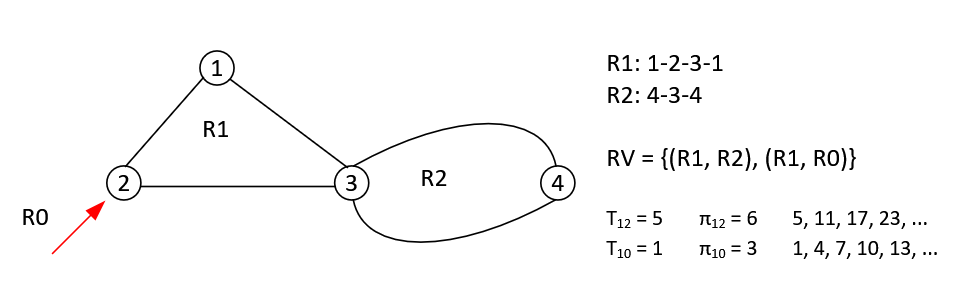
\includegraphics[scale=0.3]{Figures/SmallExaple.png}
\caption{Simple example.}
\label{ex:flow}
\end{figure}

For the MRP example from Figure \ref{ex:flow}, the associated flow network is presented in Figure \ref{patrolling}. In our example, the moment of time $T$ until the network is presented is 20. The amount of data which is collected by the robots is marked with green. \textcolor{black}{For a better readability of  Figure \ref{patrolling}}, we did not connect the green arrows to the source (as described in Section \ref{model}), but in the implementation they are connected. The decision making strategy for the robots, which is the output of the $DynFloR$ algorithm proposed in Section \ref{dynflor}, is marked with red. If an arc between two nodes $i_t$ and $j_t$ is labelled with a value $v$, it means that at time $t$ robot $R_i$ transfers to robot $R_j$ the amount $v$ of data. If the arc between $i_t$ and $i_{t+1}$ is labeled with $v$, it suggests that robot $R_i$ stores in its memory the amount of data $v$ for one unit of time (from $t$ to $t+1$).   

\begin{figure*}[!htb]
\centering
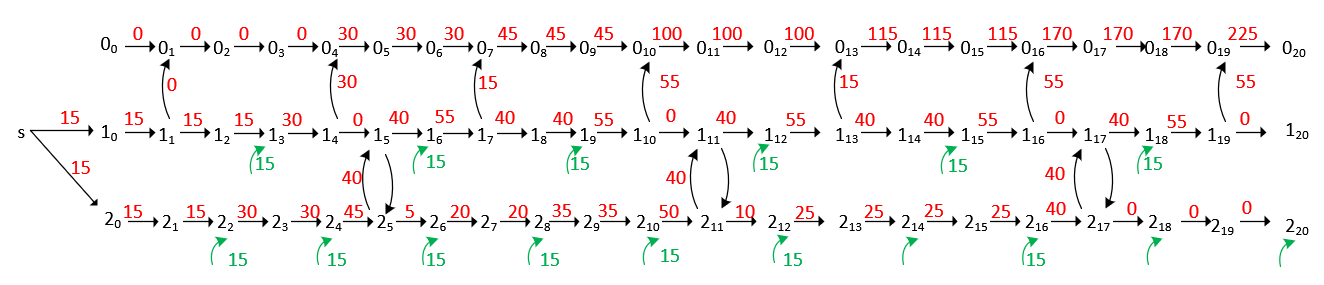
\includegraphics[scale=0.33]{Figures/FlowFinal2.png}

\caption{The dynamic network for the example from Figure \ref{ex:flow}. The decision making strategy for the robots is marked with red.}
\label{patrolling}
\end{figure*}

From Figure \ref{patrolling} we can observe that 225 units of data were transferred to the sink (robot R0) by $t = 20$. We can also observe that there are 3 green arrows (robot R2 at times 14, 18 and 20) that do not have incoming data. This data is not lost, it is stored in the memory of the robots, but since until the time limit we have set for the simulation ($t=20$) it cannot arrive to the sink, the flow algorithm does not consider it. But if we extended the time limit to include another meeting between robots R1 and R2, most of these data would arrive to the sink.

There is also the possibility to have lost data, a situation in which no matter how long we would extend the time limit, the data would never arrive to the sink. This is mainly due to the maximum memory capacity of the robots and the frequency of the collected data.    For instance, if we considered the value 40 as the maximum capacity for robot R2 (and left the other settings used for Figure \ref{patrolling} the same), by time 5, when R2 first meets R1 and has the chance to transfer data, it should have accumulated 45 units of data, which is impossible. In our model, if the robot's memory is full, the new data will not be collected (instead of overwriting existing data with the new one).

In order to determine which data is lost and which data is in the memory of a robot (and consequently will arrive to the sink in the future), we used the following method: after measuring the flow for time $Time$, as presented in Algorithm \ref{alg:dynflor}, we build a new, extended graph for time $2 \cdot Time$. In this extended graph we added the extra edges denoting new data coming from the source to the robots only until time step $Time$, so second half of the graph has no extra data coming. We measure the flow in this extended graph and the difference between the flows denotes the data that is in the memory of the robots at time $Time$ and will arrive to the sink later. We also know the total data that should enter the graph (the sum of the capacities of the outgoing arcs of the source node) and the difference between this data and the flow of the extended graph is the quantity of the data that is lost.
The robot that loses data is determined by the flow algorithm, and in the current implementation we only try to optimize the total quantity of data that arrives to the sink, and do not try to balance the lost quantities between robots.

\section{Results and discussion}\label{discussion}

In this section we present our current results obtained using the algorithm presented previously. The network flow part of our DynFloR algorithm was implemented using the Python NetworkX \cite{nx} graph library.

We performed incipient simulations on randomly generated inputs of $20$ robots with the same $MaxCapacity$ for each robot. Figures \ref{figure1} and \ref{figure2} show the evolution of the $f(T)$ and $g(T)$ objective functions for two different values of $MaxCapacity$. We observe that both functions converge to an equilibrium state and this convergence is independent of the memory capacity. Multiple random experiments confirm this.

\begin{figure*}[!htb]
\begin{minipage}{0.5\linewidth}
\centering
  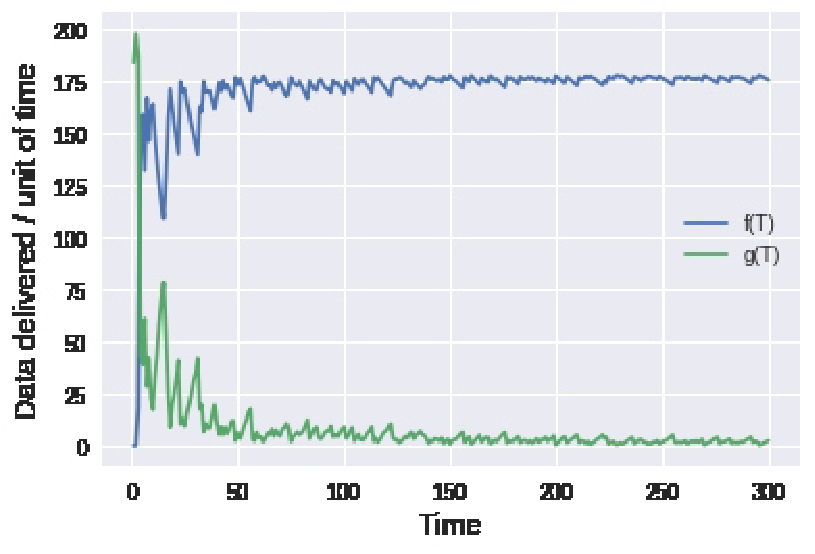
\includegraphics[scale=0.6]{Figures/graf1.pdf}
  \caption{Results for $20$ robots and $MaxCapacity=1000$. }
  \label{figure1}
\end{minipage}
\hfill
\begin{minipage}{0.5\linewidth}
\centering
  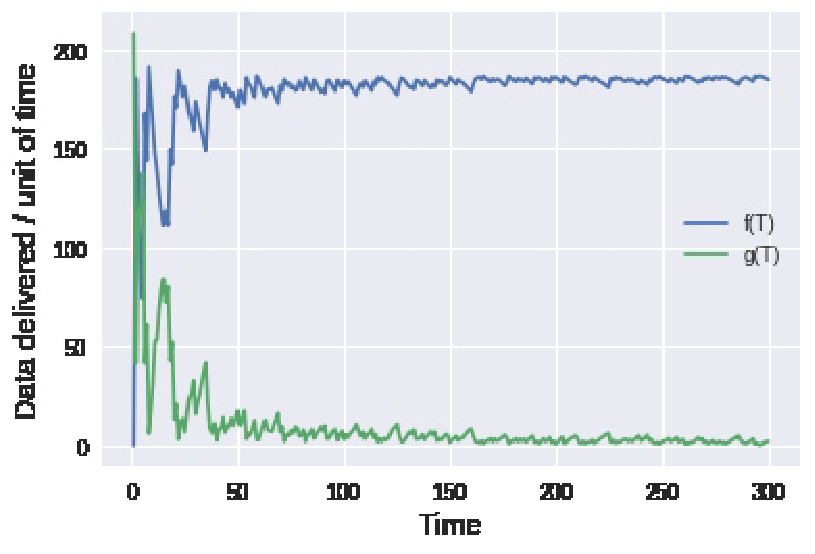
\includegraphics[scale=0.6]{Figures/graf2.pdf}
  \caption{Results for $20$ robots and $MaxCapacity=800$.}
  \label{figure2}
\end{minipage}
\end{figure*}

In order to better visualize the relation between data that enters the system, data that is currently in the memory of robots and data that is lost, we have performed some experiments using the simple example from Figure \ref{ex:flow}, setting the quantity of initial data and new data that is collected after every cycle to $15$. We have considered different values for $Time$ and $MaxCapacity$ (but considering the same capacity for both robots). The results are presented in Table \ref{table:memory}.

The value in parentheses after $Time$ represents the total quantity of data that enters the system until that time moment and which is divided into data that arrived to the sink, data that is currently in the memory of the robots, and data that is lost. We can see that as the $MaxCapacity$ of the robots increases, so does the amount that arrives to the sink and consequently the quantity of lost data decreases. From Table \ref{table:memory} it looks like setting the $MaxCapacity$ to 60 is enough to make sure that no data is lost, but in order to be certain of this, more experiments and maybe mathematical proof is necessary, because at time 20, there was no lost data for $MaxCapacity$ 55 either, but later this changed. Data that is currently in the memory of the robots is always bounded by the total memory the robots have, in our case $2 \cdot MaxCapacity$.

\begin{table}[!htb]
\small
\begin{center}
\resizebox{\textwidth}{!}{
\begin{tabular}{|c|c|c|c|c||c|c|c|c|c| } 
\hline
\textbf{Time} & \textbf{Maximum}  & \textbf{Data arrived} & \textbf{Data in} & \textbf{Lost} & \textbf{Time} & \textbf{Maximum}  & \textbf{Data arrived} & \textbf{Data in} & \textbf{Lost} \\
& \textbf{capacity} & \textbf{at sink} & \textbf{memory} & \textbf{data} & & \textbf{capacity} & \textbf{at sink} & \textbf{memory} & \textbf{data} \\
\hline \hline

\multirow{5}{*}{20 (270)} & 40 &  180   &  40  & 50  & \multirow{5}{*}{40 (420)} & 40 & 360    & 40 & 125        \\ \cline{2-5} \cline{7-10}

& 45 &   195& 45   & 30  &                     & 45 & 390     & 45    & 90        \\ \cline{2-5} \cline{7-10}

& 50 &  210& 45    & 15  &                   & 50 &     420 &  50     & 55       \\ \cline{2-5} \cline{7-10}

& 55 &  225    & 45 & 0  &                     & 55 &    450  & 55      & 20      \\ \cline{2-5}\cline{7-10}

& 60 &  240& 30   & 0    &                     & 60 &   480   & 45      &0       \\ \hline
\multirow{5}{*}{60 (705)} & 40 &  525   & 70  & 185  & \multirow{5}{*}{80 (1020)} & 40 & 730 & 40 & 250        \\ \cline{2-5} \cline{7-10}

& 45 & 570  & 75   & 135  &                     & 45 &     795 &45    &180         \\ \cline{2-5} \cline{7-10}

& 50 & 615&  80  & 85 &                   & 50 &    860 &   45   & 115      \\ \cline{2-5} \cline{7-10}

& 55 & 600 & 85& 35  &                     & 55 &   925  &  45   & 50      \\ \cline{2-5}\cline{7-10}

& 60 &  705 & 75  & 0  &                     & 60 &  990  & 30   & 0      \\ \hline
                    
 \end{tabular}}
  \caption{Quantity of data in memory, at the sink and lost, for different maximum capacities and time limits for the example from Figure \ref{ex:flow}. Initial data and new data received after every completed cycle is 15.  }
  \label{table:memory}
\end{center}
\end{table}

From Table \ref{table:memory} we can also observe that for a given $MaxCapacity$ the quantity of lost data is not double if we double $Time$. For example, for $MaxCapacity$ 50, we have 15 units of lost data after $Time$ 20, but if we double $Time$, the quantity of lost data becomes 55. We performed some experiments in order to better understand how the quantity of lost data changes if time increases, for a fixed $MaxCapacity$. In Table \ref{table:increase} we included two scenarios: the left part of the table was computed for $MaxCapacity$ 50, while the right part was computed for $MaxCapacity$ 40. For both scenarios, we computed also the rate of Lost data / Time (in the 4th and 8th column).

\begin{table}[!htb]
\small
\begin{center}
\resizebox{\textwidth}{!}{
\begin{tabular}{|c|c|c|c||c|c|c|c|} 
\hline
\textbf{Maximum}&\textbf{Time} & \textbf{Lost Data} & \textbf{Lost data / Time} & \textbf{Maximum}&\textbf{Time} & \textbf{Lost Data} & \textbf{Lost data / Time} \\
\textbf{capacity}&&&&\textbf{capacity}&&&\\
\hline \hline
&10 & 5    & 0.5 & &10 & 25 & 2.5\\ 
\cline{2-4}\cline{6-8}
&20 &  15  &  0.75& & 20 & 50 & 2.5\\ \cline{2-4}\cline{6-8}
&50 & 65    & 1.3 & & 50 & 150  & 3\\ \cline{2-4}\cline{6-8}
&100 &  155  & 1.55 & & 100 & 325 & 3.25\\ \cline{2-4}\cline{6-8}
&200& 315    &  1.575 & & 200 & 650 & 3.25\\ \cline{2-4}\cline{6-8}
&500& 815    &  1.63 & &500 & 1650 & 3.3\\ \cline{2-4}\cline{6-8}
50&1000& 1655   &  1.655& 40&1000 & 3325 & 3.325\\ \cline{2-4}\cline{6-8}
&5000 &  8315  & 1.663  & & 5000 & 16650 & 3.33\\ \cline{2-4}\cline{6-8}
&10000& 16655   &  1.6655& & 10000 &  33325& 3.3325\\ \cline{2-4}\cline{6-8}
&50000&  83315  & 1.6663 & &50000 &  166650 & 3.333\\ \cline{2-4}\cline{6-8}
&100000&   166655 & 1.66655  & &10000 &  333325 & 3.33325\\ \hline
\end{tabular}}
\caption{Progression of lost data as time increases for different $MaxCapacity$ values}
%50 (first three columns) and 40 (last three columns).}
\label{table:increase}
\end{center}
\end{table}

As expected, Table \ref{table:increase} reveals that the quantity of lost data per time significantly decreases as the maximum memory capacity of the robots increases. Additionally, as illustrated in Figure \ref{fig:lostdata}, it seems that the lost data per time converges to an equilibrium state, independent of the maximum capacity of the robots. This can be observed more clearly by running the proposed flow algorithm for more time steps, thus allowing all the data to arrive at the sink. As we have previously discussed, the data which does not arrive to the sink until a certain time limit is not necessarily lost, as it may arrive to the destination if we extend the time limit. Still, there is also the possibility to have lost data, a situation in which the data would never arrive to the sink no matter how long we would extend the time limit. Further experiments and theoretical analyses will be performed in this direction.

\begin{figure*}[!htb]
\centering
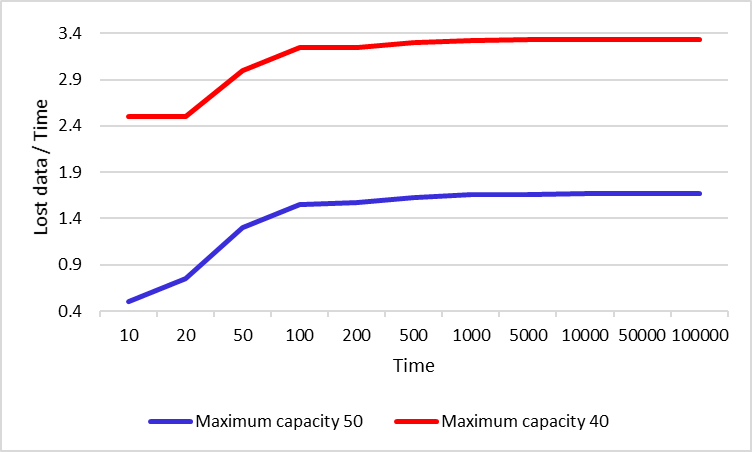
\includegraphics[scale=0.3]{Figures/Lost.png}
\caption{Variation of lost data per time for the example from Figure \ref{ex:flow}.}
\label{fig:lostdata}
\end{figure*}

\subsection{Comparison to related work}\label{compRelatedWordkDynFloR}

The literature contains various approaches related to multi-robot patrolling described in Section \ref{lr}, but we have not found approaches for optimizing data delivery in MRP.

Our work differs from the approaches described in Section \ref{lr}, as it has a different target than the previously described related work. It approaches the problem of data delivery optimization in a deterministic MRP setting using a dynamic flow based approach. As far as we know, approaches similar to $DynFloR$ do not exist in the MRP/DMRP literature. The most similar  approach to ours is the one of Liemhetcharat et al. \cite{Liemhetcharat2015}. The problem approached in the current chapter differs from the one of Liemhetcharat et al. \cite{Liemhetcharat2015}, even if both chapters are dealing with the data delivery problem. The perspectives are different, since the chapter \cite{Liemhetcharat2015} considers data delivery from a central location to several local targets, while in our chapter the perspective is the opposite one. 

A major advantage of $DynFloR$ is its polynomial time complexity, compared to the classical brute-force exponential solutions \cite{Romeo2018}. In addition, $DynFloR$ works well for dynamic data, i.e. data which continuously appear on each robot cycle. Another advantage of $DynFlor$ is that it finds the global optima, unlike the metaheuristic approaches (such as \emph{genetic algorithms} - GAs) \cite{portugal_2011}) which may provide a local optima. Besides, another difficulty when modelling the MRP using GAs relies on the chromosomes' modelling and on incorporating the continuous data collection into the model. An additional benefit of $DynFloR$ is that it can be adapted for the dynamic case of the MRP, under the same assumptions currently considered. When new targets are discovered during the dynamic patrolling problem and they are allocated to new patrolling robots, new nodes are simply added to the flow network graph $G$ and $DynFloR$ is executed again. An adaptive version of $DynFloR$ may be further investigated, with the goal of adapting the solution provided by $DynFloR$ instead of running it from scratch when new cycles to be patrolled are discovered.  

One of the current limitations of $DynFloR$ is given by the assumption regarding the periodicity of the robots' meetings. In the general case, in real DMRP scenarios,  instead of having initial meeting times and meeting periods, there is an uncertainty of the meetings as the robots' speed is not constant. For offering a solution to the data delivery optimization for the general case, \emph{reinforcement learning} would be further investigated  for adapting the robots'  decision making policy to the uncertainty of the world.  


\section{Conclusions and future work}\label{conc}

In this chapter we have investigated the data delivery optimization in a simplified setting  for the \emph{multi-robot patrolling} problem in which the environment is deterministic. We introduced accordingly a centralized and offline approach $DynFloR$ based on flows in dynamic networks. The goal of $DynFloR$ is to determine the robots' policy for maximizing  the quantity of data delivered to a base station in a given time, assuming that the robots are continuously collecting data during the patrolling. The more general aim of the research initiated in this chapter is to explore the general case of the problem  of optimizing the data delivery in DMRP when the environment is non-deterministic and uncertain (i.e. there are communication failures). 

Further work will extend the experimental evaluation and theoretical analysis of $DynFloR$ in order to better assess its performance. We also aim to decentralize the decision making process and to incorporate uncertainty in the communication between robots.  An extension of $DynFloR$ to an online approach and the incoming data model to an irregular one will be subjects to future developments. In order to achieve these goals, a \emph{reinforcement learning} perspective will be considered. 


\chapter[A RL Approach for Data Delivery Optimization]{A Reinforcement Learning Approach for Data Delivery Optimization in Multi-Robot Network Patrolling}
\label{rl}
This chapter aims to illustrate the feasibility of a \emph{reinforcement learning} approach to optimizing the data delivery in MRP. The $\mathit{DynFloR}$ method showcased in \emph{Chapter 2} lacks one key asset in order to be fully reliable, that being \emph{learning} how to react in uncertain conditions and dynamic environments.

When thinking about the nature of learning, perhaps several examples of instances come up in our minds when we learn something simply by interacting with an environment, and receiving a positive or negative reward when making a decision. One issue encountered in \emph{RL} modelling of complex environments is the exponential pool of states in which the environment can be found, and the large number of actions that the robots can perform at any given time.

\par The study conducted in this chapter consists in a new approach, based on \emph{Q-learning}, under the assumptions defined in \emph{Chapter 2} (i.e. the environment is deterministic, the network of robots is centralized and offline, and the robots have periodic meetings). Experiments and simulations carried out on several synthetic and randomly generated examples prove that the \emph{RL} approach for the data delivery optimization in MRP is feasible.

\par The rest of the chapter is structured as follows. The \emph{reinforcement learning} approach for data delivery optimization in a deterministic setting of the MRP is introduced in Section 3.1. Section 3.2 is concerned with the advantages and limitations of the proposed model, while Section 3.3 contains the conclusions of the chapter and possible future developments of this work.
%RL MODEL
\pagebreak

\section{The proposed RL methodology}

This section introduces a centralized and offline \emph{RL} approach for data delivery optimization in a deterministic setting of the MRP, being applicable in a deterministic setting of DMRP, with minimal improvements.


\subsection{The DronemRL model}\label{rlmodel}

The problem approached in this chapter is the same problem defined in \emph{Chapter 2}, so we will focus solely on the \emph{reinforcement learning model}.
\subsubsection{The action model}

For this specific problem an action was defined to be a list $X=[x_{1}, x_{2},\dots,x_{k}]$, where $k=\frac{n(n-1)}{2}$. There are $\frac{n(n-1)}{2}$ elements in our list, because we have  $\binom{n}{2}$ ordered pairs of robots $(R_{i}, R_{j})$ with $i < j$.
That being said an element at any given position $p, 1 \leq p \leq k$ in our action list describes the quantity of data exchanged by robots $(R_{i}, R_{j})$, $i < j$, this quantity is bounded by robot's $MaxCapacity$ meaning that there cannot be transfers between $(R_{j}, R_{i})$ if $j > i$, so in order to address this problem the domain of values for $x_{i} \in X$ is $\{0, 1,\dots, 2\cdot MaxCapacity\}$.
Therefore $x_{i} \in X$ has the following meaning:

$$
x_{i} = \begin{cases} 
    \text{transfer $x_i$ data from $R_i\rightarrow R_j$}, & 0\leq x \leq MaxCap \\
     \text{transfer $x_i - MaxCap$ data from $R_j\rightarrow R_i$}, & MaxCap < x\leq 2\cdot MaxCap\\
    \end{cases}
$$


\noindent Every action of the environment can be thought to be an element of the following cartesian product:
$$ A = \varprod_{i=1}^{\frac{n(n-1)}{2}} A_i$$
where $A_{i}=\{0, 1, 2,..., 2\cdot MaxCapacity\}$ meaning that there are  $(2\cdot Maxcapacity)^{\frac{n(n-1)}{2}}$ actions in total.
Thus it can already be seen that the action space is extremely large. For example if we have $10$ robots and \emph{MaxCapacity} $= 10$, we would have $20^{45}$ actions. This problem is addressed in \cite{dulacarnold2015deep}, by having an actor-critic model, where the actor applies actions and the critic learns to generate actions in some proximity of the current action using some defined mathematical norm. Even though this approach solves the problem of very large action spaces, there is still the problem that at any given time there is a small number of valid actions to choose from and most of the time the critic will generate invalid values, hence determining the model to apply only invalid actions. 

\par In order to address the issue of large state and action spaces the classic Q-learning algorithm, from Section \ref{qLearningAlgo} was modified, to initialize and update the Q-table in a dynamic way (i.e. $states$ are added in the Q-table only when they are encountered, not at the beginning of the algorithm) and variation of the Q-learning algorithm will be called \emph{DronemRL}.

\subsubsection{The state model}
For the state model of the environment, it is enough to know the quantity of data each robot holds, the current time step and the position of each robot.
Therefore, a state is represented as a list $S=[s_1, s_2, \dots, s_{2n + 1}]$, where elements $[s_1, \dots, s_n]$ represent the quantity of data of each robot, $s_{n + 1}$ is the current time step and $[s_{n + 2}, \dots ,s_{2n + 1}]$ represent the current position of each robot.

\subsubsection{The reward function}
After trying several types of reward functions, the one which proved to be the best in practice is defined below: 

\begin{itemize}
  \item If the action is invalid (i.e. $R_{j}$ cannot receive the data transferred by $R_{i}$ or $R_{i}$ does not have enough data in its memory), or there is an invalid meeting return a penalty reward of $invalidActionReward=-10^{7}$.
  \item If the chosen action is to do nothing when it is not the case (i.e. the robots can exchange data) reutrn $\frac{2}{3}\cdot invalidActionReward$.
  \item Else add  $dataTrasferred$ to the reward value for each transfer to $R_{0} \text{ (the sink)}$ and  $1$ for any other valid transfer.
\end{itemize}

The reward function is defined in such a way that if our model chooses an invalid action, it receives a large negative reward in order to adjust the $Q(s,a)$ value for that action in that particular state, thus next time when our model is in state $s$ this invalid action won't be chosen. Also the reward function encourages the model to select actions which facilitate transfer of large amount of data to our \emph{sink}. In \emph{RL} the reward function is the core element of $learning$ because it must be defined in a way that it emphasizes the environment characteristics. The best known reward function \cite{rsab} is the one which gives $-1$ reward for every action and $0$ for terminal actions, it is guaranteed that the model will learn to choose the best actions in every state, but the drawback is that the learning time required for such a reward function is tremendously large, therefor impractical for many complex environments such as ours.

\subsubsection{$DronemRL$ algorithm}\label{rlalgo}
After constructing the environment having the properties stated in Section \ref{rlmodel} we train the reinforcement learning model for a number of \emph{episodes}. For every episode of the training process we apply the update rule defined in Section \ref{qLearningAlgo}, based on \emph{Bellman's equation}. One important aspect to take into consideration about this algorithm is that, we do not initialize the entire Q-table (i.e. a matrix storing every possible $(state,action)$ pairs), instead we initialize the Q-table to be empty and only add new states and actions dynamically when we encounter them.

The pseudocode for the dynamic Q-table update is presented in Algorithm \ref{alg:qUpdate} while the DronemRL algorithm is given in Algorithm \ref{alg:dronemrl}.

\begin{algorithm}[!htb]
\caption{Function $UpdateQTable$}\label{alg:qUpdate}
\begin{algorithmic}
\Function{$UpdateQTable$}{$Q, state, action, reward, newState, \alpha, \gamma$}
\Ensure{Dynamically updates the Q-table based on \emph{Bellman's equation} }
\If{$newState \notin Q$}
    \State{//if the new state is not in the Q-table add it}
    \State{$addStateInQTable$($newState$)}
\EndIf
\State{//get the maximum Q-value of the new state}
\State{$maxQFuture \leftarrow max$($Q(newState)$)}
\State{//get the current Q-value}
\State{$currentQValue \leftarrow Q(state, action)$}
\State{//update the Q-table}
\State{$Q(state,action) \leftarrow Q(state, action) + \alpha \cdot (reward + \gamma \cdot maxQFuture)$}
\EndFunction

\end{algorithmic}
\end{algorithm}

\begin{algorithm}[!htb]
\caption{Algorithm $DronemRL$} \label{alg:dronemrl}
\begin{algorithmic}
\State{\textbf{Algorithm} DronemRL is:}
\State{//determines the optimal policy for the robots data delivery}
\Require{$env, nEpisodes, \epsilon, decay, maxNumOfSteps, \alpha, \gamma$ {\rmfamily - the input parameters for the $DronemRL$ algorithm}}
\Ensure{returns the Q-table containing Q(s,a) values as described in Section \ref{qLearningAlgo} }
\State {//initialize empty Q-table}
\State{$Q \leftarrow emptyQTable$()}
\State{//applies the Q-learning algorithm}
\For{$episode \gets 0, nEspisodes$}
\State{//sets the reward for current episode to 0}
\State{$episodeReward \leftarrow 0$}
\State{//the current episode is not done}
\State{$done \leftarrow false$}
\State{//sets the environment to its initial state}
\State{$state \leftarrow reset$($env$)}

\Repeat
\State{$action \leftarrow selectAction$($\epsilon$,$state$)}
\State{//applies action to the environment}
\State{$actionResult \leftarrow step$($action$)}
\State{//gets the new state, the reward of applying the action and if the new state is terminal }
\State{$newState \leftarrow getState$($actionResult$)}
\State{$reward \leftarrow getReward$($actionResult$)}
\State{$done \leftarrow getDone$($actionResult$)}

\State{$episodeReward \leftarrow episodeReward + reward$}


\State{//if the episode is not done (i.e. we are not in a terminal state, and we have not reached the maximum number
of steps per episode}
\If{$done \neq true$}
\State{//updates the Q-table}
\State{$UpdateQTable$($Q$, $state$, $action$, $reward$, $newState$, $\alpha$, $\gamma$)}
\Else
\State{$time \leftarrow getTime$($newState$)}
\If{$time = maxNumOfSteps$}
\State{//if we reached the end of the episode because we've used the maximum number of steps, penalize the action}
\State{$Q(state, action) \leftarrow -1$}
\Else
\State{$Q(state, action) \leftarrow reward$}
\EndIf
\EndIf
\State{$state \leftarrow newState$}
\Until{$done=true$}
\EndFor
\end{algorithmic}
\end{algorithm}

\newpage
\section{Results and discussion}
In this section the results obtained using the proposed algorithm are showcased. All operations involving the manipulation of Q-tables were performed using the Python Numpy \cite{numpy} numerical computation library.
\par The algorithm was tested against several randomly generated environments having 3 robots with the same $MaxCapacity=10$ for each robot. Figure \ref{minReward} and Figure \ref{maxReward} show the evolution of the minimum and maximum reward per $50$ episodes for a total number of $50000$ episodes.
\begin{figure*}[!htb]
\begin{minipage}{0.5\linewidth}
\centering
  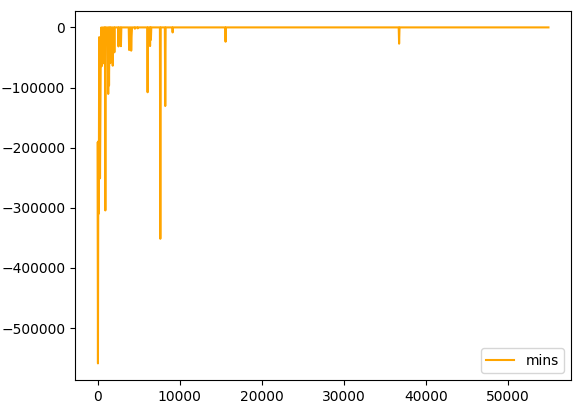
\includegraphics[scale=0.5]{Figures/minsBigEnv.png}
  \caption{Results for $3$ robots and $InitialMemory=4$}
  \label{minReward}
\end{minipage}
\hfill
\begin{minipage}{0.5\linewidth}
\centering
  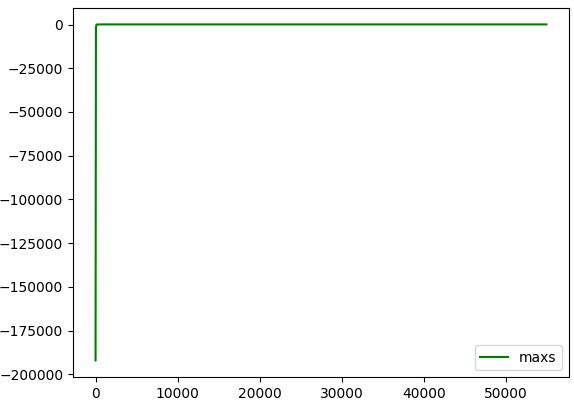
\includegraphics[scale=0.5]{Figures/maxBigEnv.png}
  \caption{Results for $3$ robots and $InitialMemory=4$}
  \label{maxReward}
\end{minipage}
\end{figure*}

\par It can be seen from the figures above that the algorithm reaches convergence well before 50000 episodes. The Q-learning model quickly identifies the optimal data transfer policy between robots. Given the fact that the initial memory of the robots is $4$ and the $MaxCapacity$ for all robots is $10$, one robot $R_i$ can accommodate all the memory initially contained in the memory of $R_j$, explaining the rapid convergence of our algorithm on this particular case.
\par However, tests were ran on more complex environments, Figure \ref{allRewards} depicts the minimum, maximum and the average reward per $50$ episodes on an environment having 3 robots, with $MaxCapacity = 9$, but having $initialMemory = 7$. In this case the transfer policy is more complex because when two robots meet for the first time they cannot exchange all their data, as they need to figure out that they can only send $2$ units of data between them.

\begin{figure*}[!htb]
\centering
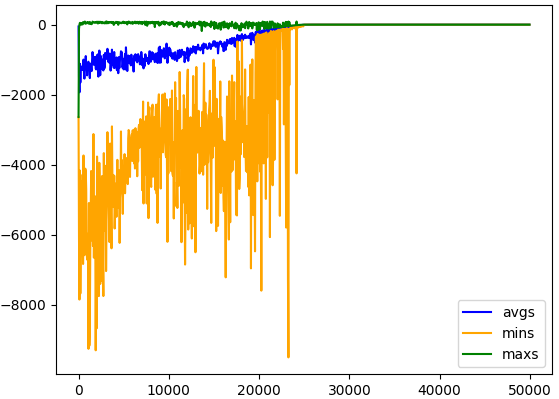
\includegraphics[scale=0.7]{Figures/plotBigEnv.png}
\caption{Results for 3 robots and $MaxCapacity=9$, $InitialMemory=7$}
\label{allRewards}
\end{figure*}

\par It can be observed that the algorithm converged slowly on this more complex environment and the main factor which contributes to the convergence is the ratio between $MaxCapacity$ and $InitialMemoroy$. Therefore, the following question arises: Given $P=\frac{InitialMemory}{MaxCapacity}$ will the algorithm eventually converge? In order to provide an answer, several tests were made with different ratios and results can be seen in Figure \ref{convergenceFig}

\begin{figure*}[!htb]
\centering
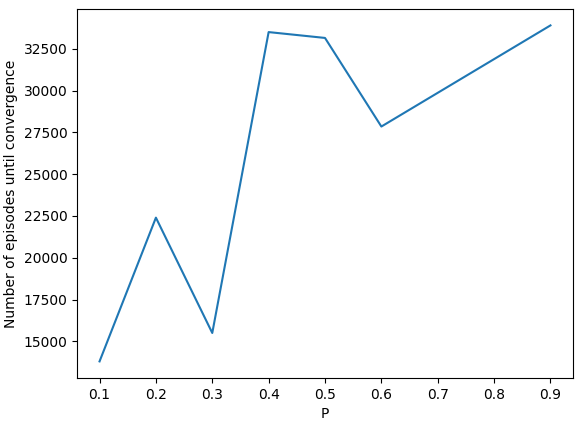
\includegraphics[scale=0.7]{Figures/convergenceGraph1.png}
\caption{Convergence graph with respect to $P$}
\label{convergenceFig}
\end{figure*}

As expected, Figure \ref{convergenceFig} reveals that eventually our algorithm convergence independent of the ratio $P=\frac{InitialMemory}{MaxCapacity}$ with linear dependence on on some intervals.


\subsection{Comparison to related work}
As it was stated in Section \ref{compRelatedWordkDynFloR}, no approaches for optimizing data delivery in MRP were found, but techniques for similar problems will be discussed.

Because classical RL algorithms are limited due to the exponential number of states and actions, we will focus on approaches oriented on \emph{DeepQ-learning}. In Deep Q-learning instead of having a Q-table in memory for storing the Q-values for every pair $(s,a)$ where $s \in S$ - the set of total States and $a \in A$ - set of total actions, we have a neural network which will $predict$ our QValues as seen in Figure 3.1.

\begin{figure*}[!htb]
\centering
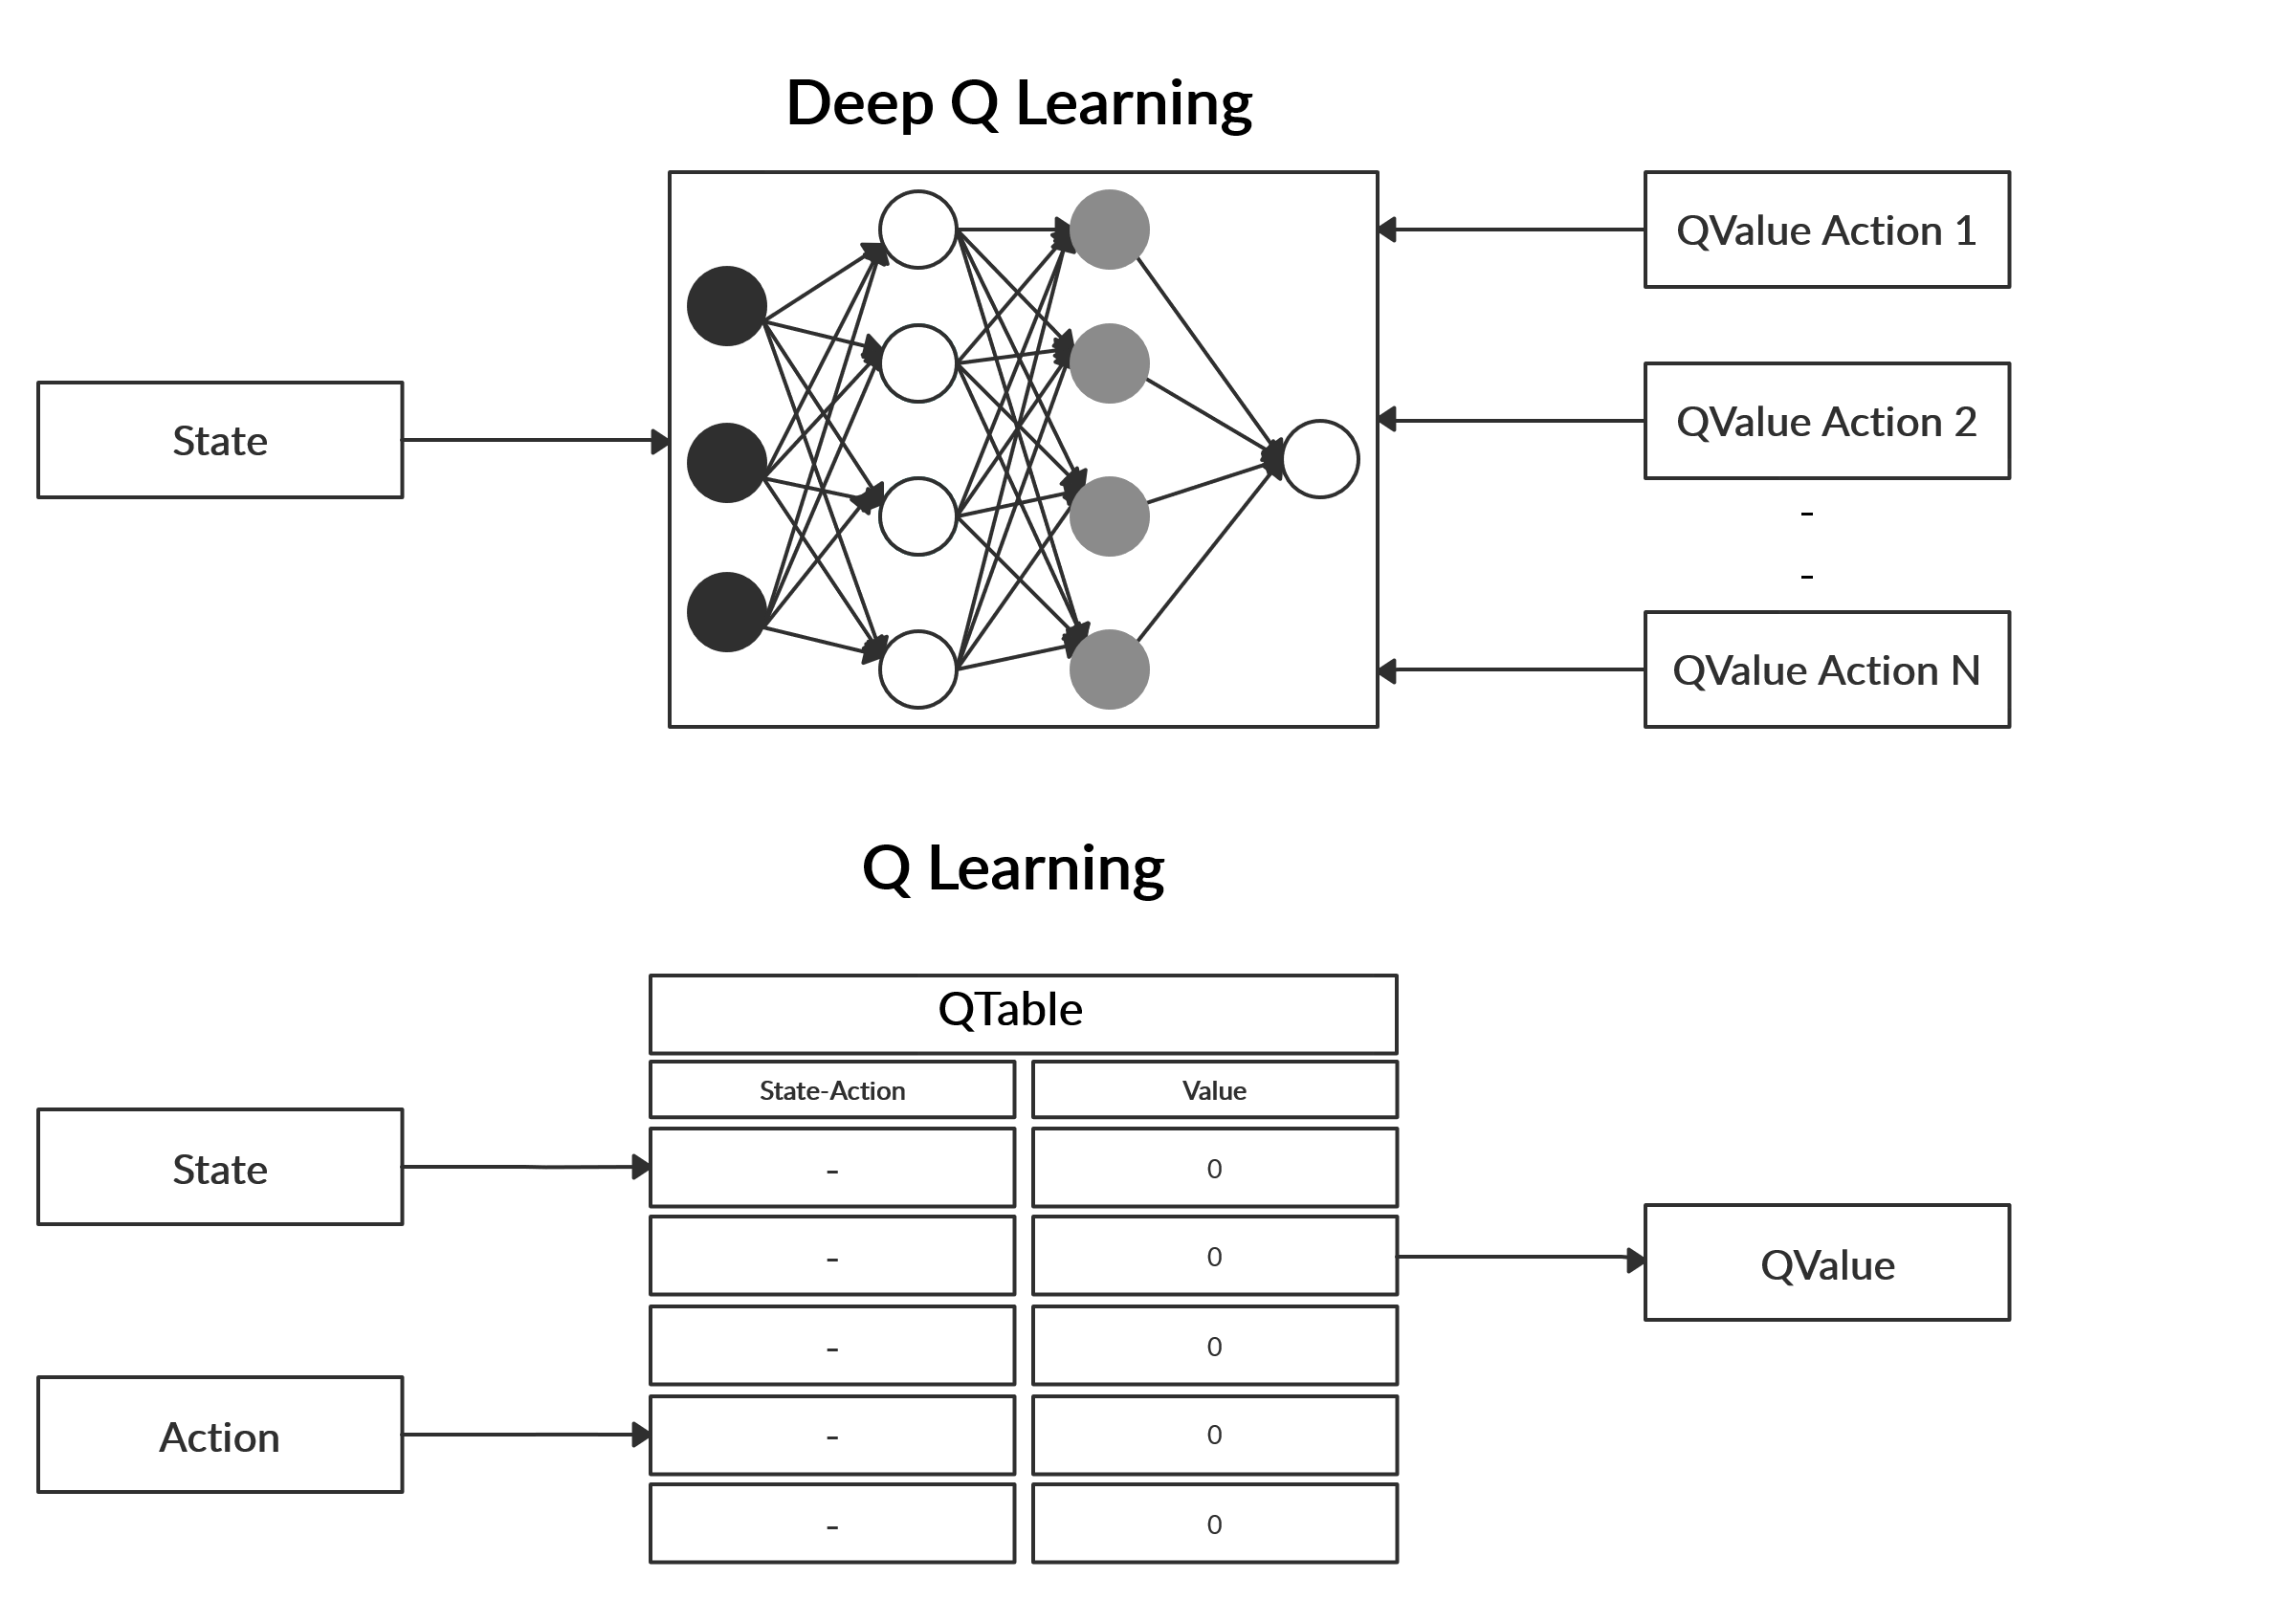
\includegraphics[scale=0.19]{Figures/QLearningvsDQN.jpg}
\caption{Classic Q-learning vs Deep Q-learning}
\label{fig:qlearningvsDQN}
\end{figure*}

\par One widely used Deep Q-learning (DQN) architecture is the one presented in \cite{dulacarnold2015deep}, also called Deep Determnistic Policy Gradient (DDPG), based on the actor critic model discussed earlier. This architecture is based on two Neural Networks, one is the actor and the other one is the critic. These networks compute action predictions for the current state and generate a temporal-difference error signal at each step. The input of the actor network is the current state, while the output is a single real value representing an action chosen from a \emph{continuous} or large discrete action space. The output of the critic is simply the Q-value of the current state and action supplied by the actor. The deterministic policy gradient theorem \cite{dpgTheorem} provides the update rule for the weights of the actor network while the critic network is updated from the gradients obtained from the temporal difference error signal.
While this approach gives good results it is often hard to find a suitable modelling for the MRP problem because of the high complexity of the environment. \\
\par Another way of tackling the training in environments with large number of actions and states is using Multi Agent approaches (every agent develops its own policy and learns how to cooperate with others) even though algorithms using this approach are notoriously unstable to train. However the OpenAI research team managed to come up with a feasible and robust approach \cite{lowe2017multiagent} by extending the actor-critic model. In the Multi-Agent DDPG (MaDDPG) OpenAI adapted the above DDPG algorithm for multi agent environments. It uses a decentralised actor, centralised critic training but during execution agents select actions relying only on their own state. This helps in easing the training as the environment becomes more stationary for each agent and the number of states and actions for each agent decreases exponentially. A diagram of the algorithm can be found in Figure \ref{fig:maddpg} \cite[Figure-1]{lowe2017multiagent}

\begin{figure*}[!htb]
\centering
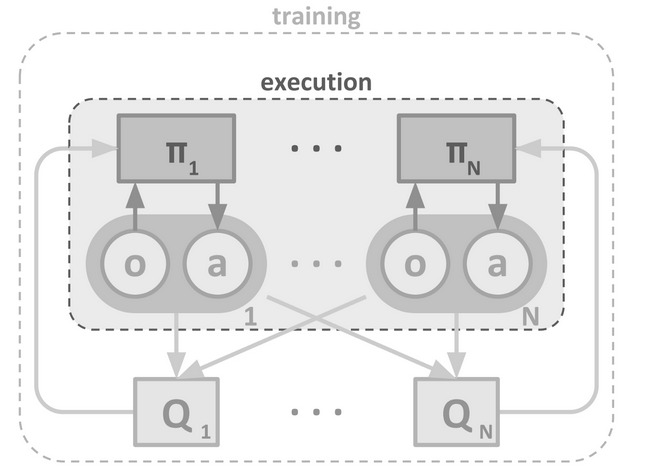
\includegraphics[scale=0.4]{Figures/maddpg.jpg}
\caption{Multi-Agent DDPG.}
\label{fig:maddpg}
\end{figure*}

\section{Future work}
In this chapter we have investigated the \emph{reinforcement learning} approach for the data delivery optimization problem in a simplified setting for the \emph{multi-robot patrolling} problem in which the environment is deterministic. Also we have introduced our centralized and offline approach whose goal is to maximize the quantity of data which arrives to our station (\emph{sink}). The aim of the above study was to prove that a \emph{reinforcement learning approach} is feasible.
\par Future work will include more rigorous testing and increase in performance. We also aim to transform the centralized system into a multi-agent system by using the approach defined in \cite{zhang2019multiagent}, this would reduce the state and action space exponentially, while increasing the performance of the system. Another enhancement which can be added to our approach is integrating the DDPG algorithm discussed earlier, which would certainly increase the performance, but our ultimate goal is to use the MaDDPG approach as it is considered to be state of the art (SOTA) when it comes to multi agent reinforcement learning. Using the MaDDPG would be suitable for the Data Delivery Optimization problem in the MRP, having each robot learn its own policy while learning to cooperate with others in training, with minimal state and action spaces, further improving the work done by \emph{DynFloR}.

%\include{Gym_env}

\chapter{A Software Solution for the Patrolling Problem}
\label{softwareApplication}

This chapter proposes a web application called \emph{Dronem Web}, based on the \emph{DronemRL} algorithm. The purpose of this platform is to facilitate a way to create, train and share results on multi-robot patrolling problems in the research community. 

\par This application represents an element of originality, as to the best of our knowledge there is no system currently available for manipulating and analyzing MRP environments. One of the strongest points of the proposed software solution is the possibility to fetch already trained cloud \emph{reinforcement learning} Q-tables for different environments, in order to further use them in real applications. 

\par Several popular and highly optimized frameworks were used for building this application on both \emph{backend} and \emph{frontend}, such as OpenAI for creating and managing the MRP environments, Django and Django Rest Framework for managing user and environment data, and ReactJS for creating the application layout and handling user interactions with the application. All this frameworks and libraries will be further detailed in this chapter. 

\par The remainder of chapter is structured as follows. In Section \ref{softDev} we make an analysis of the proposed application from a software development point of view. Section \ref{softOpenAI} shows how the MRP environments are created using the \emph{OpenAI Gym} \cite{brockman2016openai} framework, while in Sections \ref{BE} and \ref{FE} the main \emph{backend} and \emph{frontend} technologies are discussed. Implementation details and design choices are highlighted in Section \ref{implementation} and a user manual is proposed in Section \ref{userManual}. Towards the end of the chapter, some conclusions are drawn in the form of a brief discussion in Section \ref{softDiscussionn}, and finally, possible future enhancements are presented in Section \ref{futureEnh}.
 
\newpage
\section{Software development}\label{softDev}
Software development \cite{ibmSoftDev} implies all the necessary activities regarding  creation, testing and deployment of applications or other types of software. When developing an application a series of activities need to be taken into consideration in order to minimize the possibility of developing applications containing bugs, this series of activities is called a \emph{software development process} \cite{thePragmaticProgrammer}. 
\par The most important activities in Software development are the following:
\begin{itemize}
    \item Identify the need for creating the application.
    \item Planning - discovering the requirements of the application and its functionalities.
    \item Designing - creating a high-level design of the application (main modules, packages, entities, what kind of data will be managed by the application)
    \item Implementation - writing the code of the application.
    \item Testing - ensuring that the application behaves as expected according to the requirements.
    \item Documenting - writing specification for modules and packages easing maintainability of the code and extending the application.
    \item Deployment and maintenance - releasing the application and correcting any error which may appear in the future.
\end{itemize}

\par The need for Software development comes as a natural consequence of the fact that the code is written by humans, making it unreliable, hence a methodology needs to be followed in order to ensure that major bugs do not appear, and minor bugs are identified quickly and fixed. One good example of a disaster which occurred due to a major bug is The Patriot Missile Failure \cite{badBugs}, where on $25^{th}$ of February 1991, 28 American soldiers died because of a floating point arithmetic error.

\subsection{Analysis and design}\label{ad}
This subsection is focusing solely on the methodology defined in Section \ref{softDev}
\subsubsection{The necessity of this application}
While reading papers about different types of MRP problems, it was noticed that there is no application where, as a user, you can  create your own environments and try to apply different operations on them, therefore, an application capable of managing, analyzing MRP environments and sharing results is needed. Also due to the fact that MRP problems have high applicability in real life scenarios such as smart surveillance systems, this application can also serve as a tool to design such useful systems and test their capabilities.

\subsubsection{Planning}
In the planning phase, also known as \emph{collection of requirements}, we have gathered the main functional requirements of the application with the help of a use case diagram which can be observed in Figure \ref{fig:usecase}


\begin{figure*}[!htb]
\centering
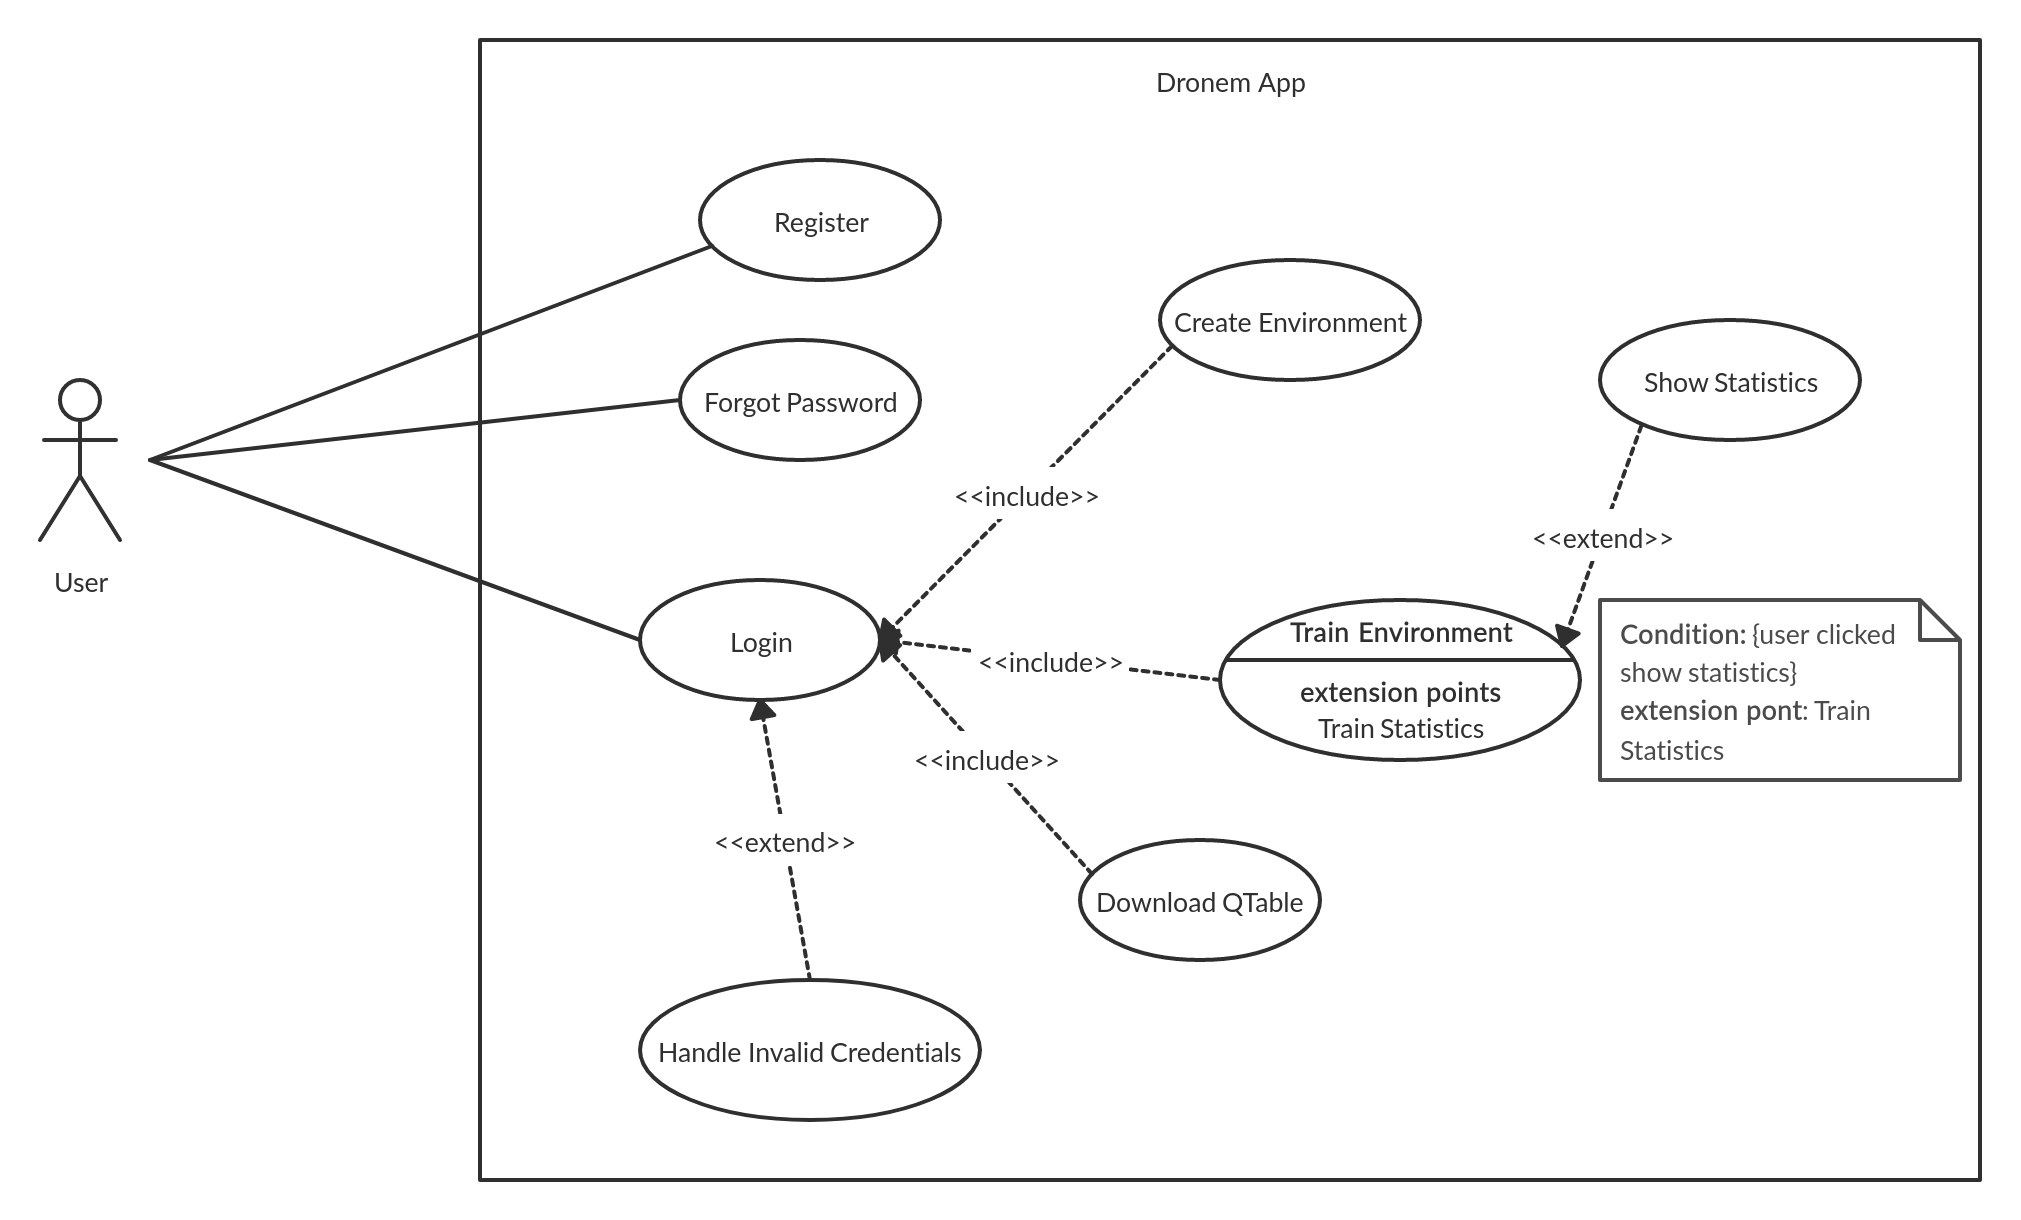
\includegraphics[scale=0.2]{Figures/UseCaseDronemRLFinal.jpg}
\caption{Use case diagram for Dronem web application}
\label{fig:usecase}
\end{figure*}


From the diagram above we can already identify the user as being the only actor of our application and the following use cases:
\begin{itemize}
    \item Register - complete registration flow for becoming a user in the Dronem Web application.
    \item Login - Authentication functionality which provides access to the core features of the application.
    \item Handle Invalid Credentials - verification of user input at login.
    \item Create Environment - use case for creating and managing MRP environments.
    \item Download QTable - possibility to download trained Q-ables for different environments.
    \item Forgot password - resetting password when a user requests it.
    \item Train Environment - possibility to train a MRP environment.
    \item Show Statistics - displaying training statistics for any environment.
\end{itemize}

One other important aspect to note is that, any use case which implies manipulating data, includes \emph{Login} and also, the \emph{Show Statistics} use case makes no sense if an environment was not trained at least once (because until the first training of the environment, there are no statistics)

\subsubsection{Design}
After the \emph{planning} phase where functional requirements were collected, a preliminary model of the main entities and the relationship between them was derived, following the Unified Model Language(UML)\cite{uml} standard, resulting in a conceptual model which can be seen in Figure \ref{fig:conceptualModel}

\begin{figure}[!htb]
    \centering
    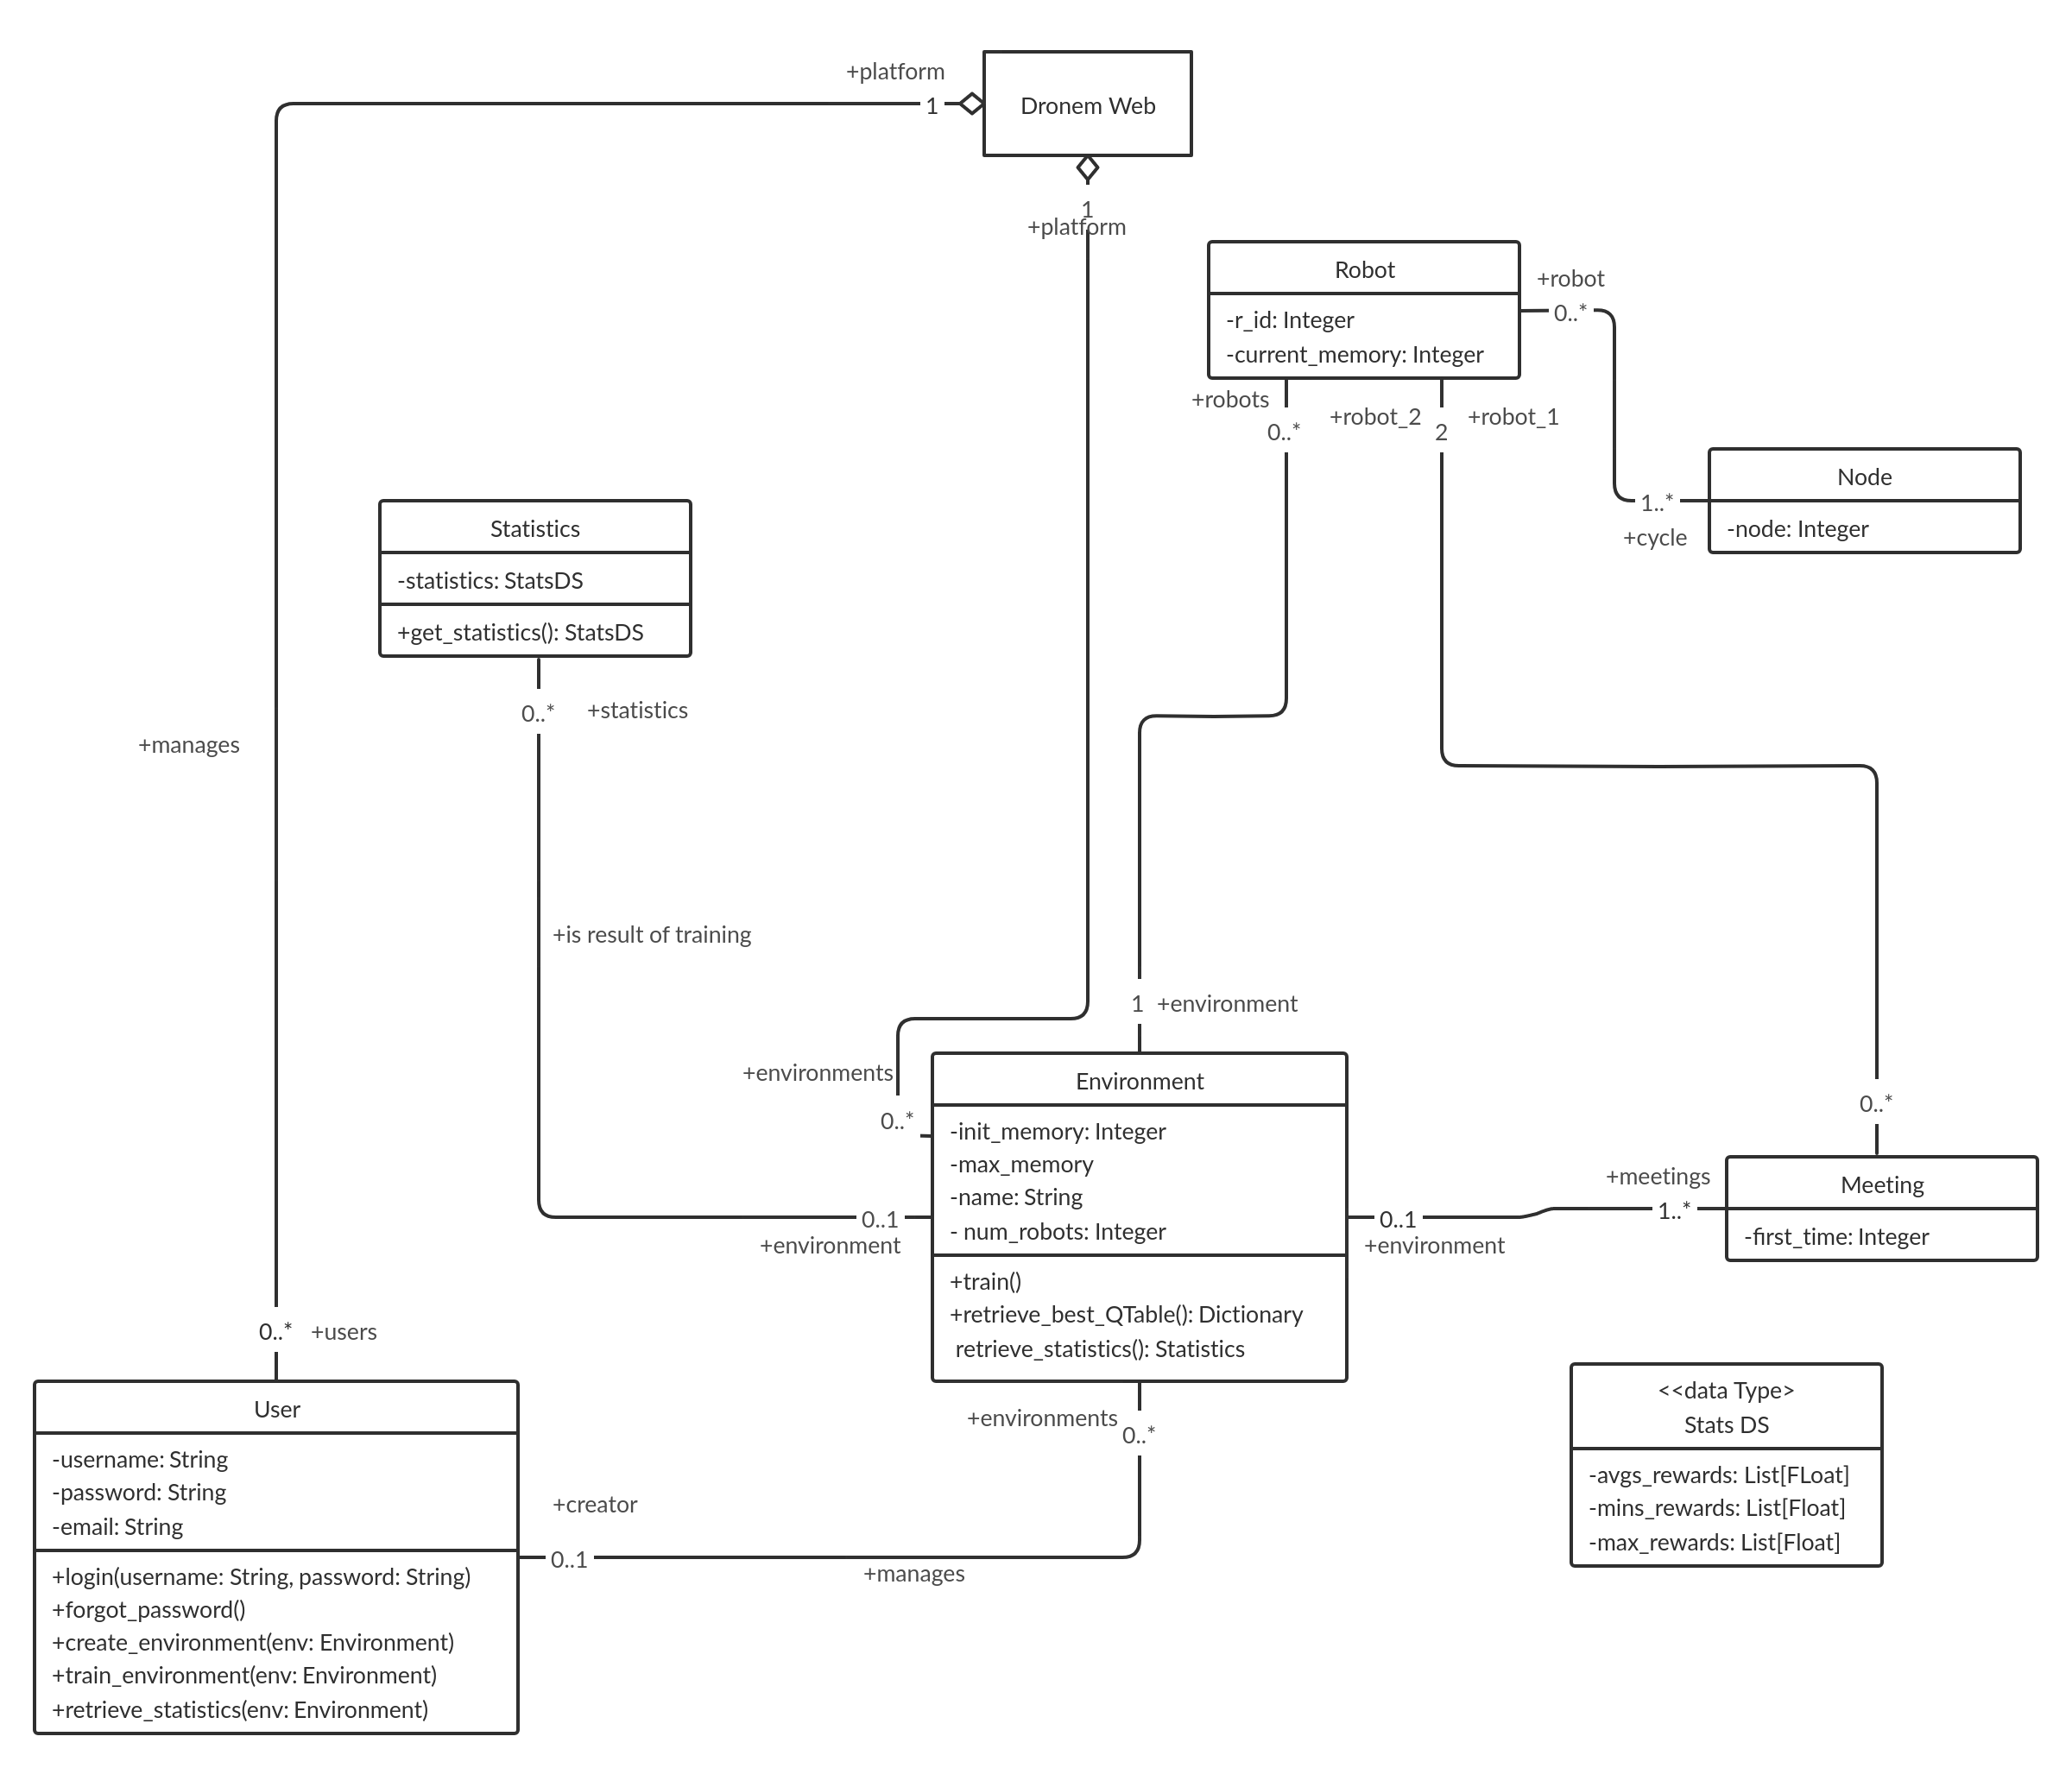
\includegraphics[scale=0.19]{Figures/conceptualModel.jpg}
    \caption{Dronem Web conceptual model}
    \label{fig:conceptualModel}
\end{figure}{}

It is known that one of the biggest problems of software development is the defective communication between clients and developers \cite{communicationProblems}, as usually the actual people who write code are not directly interacting with the client. The conceptual model diagram is an important tool which tries to solve this problems, since it eases the communication between the developers and the client by highlighting the main entities of the application and the interactions between them.
Of course, because diagram presented in Figure \ref{fig:conceptualModel} is just an intermediate step in designing the application, it is not detailed enough in order to start writing code, thus a refinement process was needed in order to obtain the final class diagram which can be viewed in Figure \ref{fig:refineDiag}

\begin{figure}[!htb]
    \centering
    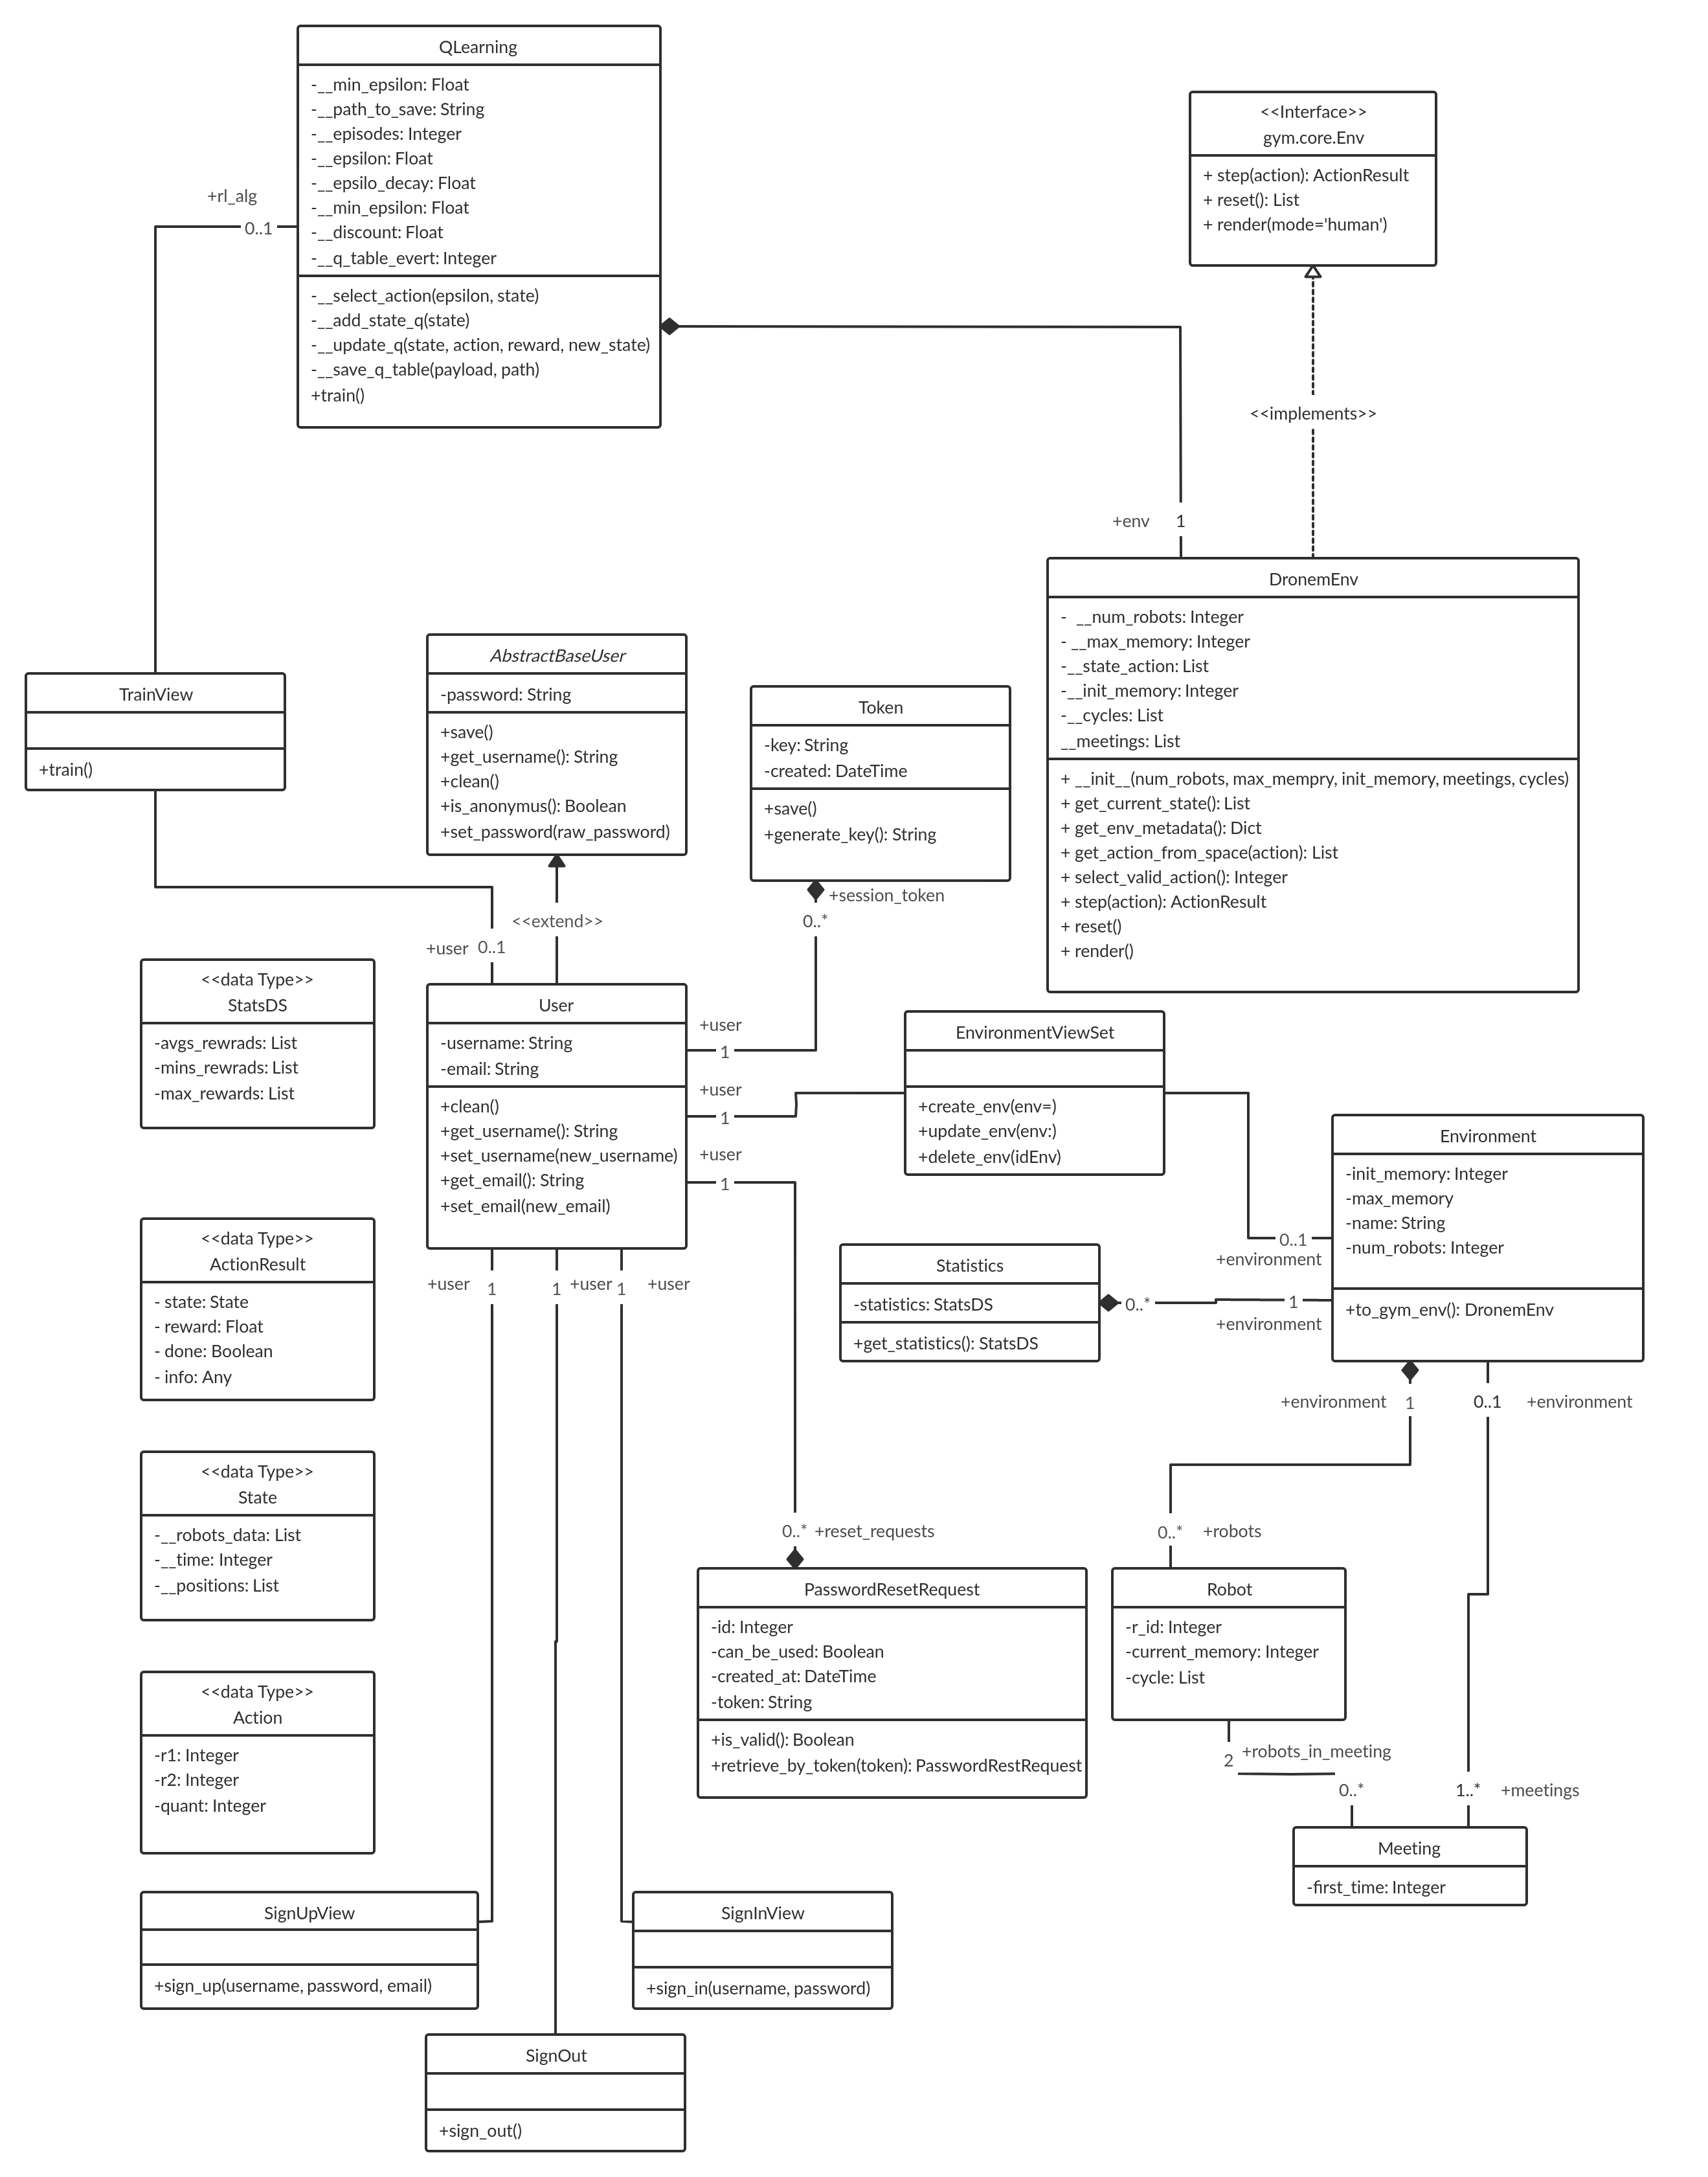
\includegraphics[scale=0.18]{Figures/umlComplete.jpg}
    \caption{Dronem Web refined UML diagram}
    \label{fig:refineDiag}
\end{figure}

\newpage
Having the refined UML class diagram we started implementing the main features of the application. More implementation details together with the next steps in the software development methodology will be outlined in the next sections.

\section{OpenAI}\label{softOpenAI}

 \emph{OpenAI Gym} \cite{brockman2016openai} is a \emph{python} toolkit for reinforcement learning environments which exposes a common interface and an website where researchers can share and compare their results. Reinforcement learning assumes that there is an agent which is situated in an environment. Each step, the agent takes an action, and it receives an observation and reward from the environment. A RL algorithm seeks to maximize some measure of the agent’s total reward, as the agent interacts with the environment. In the RL literature, the environment is formalized as a partially observable Markov decision process \cite{rsab}. OpenAI Gym focuses on the episodic setting of reinforcement learning, where the agent’s experience is broken down into a series of episodes. In each episode, the initial state of the agent is randomly sampled from a distribution, and the interaction proceeds until the environment reaches a terminal state. The goal in episodic reinforcement learning is to maximize the expectation of total reward per episode, and to achieve a high level of performance in as few episodes as possible.


\subsection{The Dronem environment}\label{gymInterface}

The OpenaAI Gym environment for our reinforcement learning model \emph{(Dronem environment)} is constructed upon  the Gym architecture\cite{brockman2016openai}, which is based on the following interface:
\begin{itemize}
  \item \textit{env.reset()} which resets the environment to its initial state;
  \item \textit{env.step(action)} which applies an action to the environment and returns back the new \emph{state} of the environment as an \emph{observation}, a variable called \emph{done} which tells if the episode should end and the \emph{reward} for applying the given action;
  \item \textit{env.render()} which renders the environment;
\end{itemize}


\par As we can see in Figure \ref{fig:dronemEnvPipeline} the life cycle of a Gym Environment is highlighted, by first starting the environment when calling $env.reset()$, then the environment expects an action in order to call $env.step()$, after that we analyze the new state and reward to draw conclusions about our actions. After calling the $env.step()$ function, if the $done$ variable is true, we then stop the Dronem environment.

\par Following the interface defined in Section \ref{gymInterface}, it was easy to design and implement the architecture from Figure \ref{fig:dronemEnvGym} in order to obtain a reinforcement learning environment following the specification of the problem defined in Chapter \ref{flow}. We can observe that we are not limited in the number or type of our parameters and functions used in the environment, as long as we implement the functions in the \emph{Gym} interface.

\begin{figure}[!htb]
    \centering
    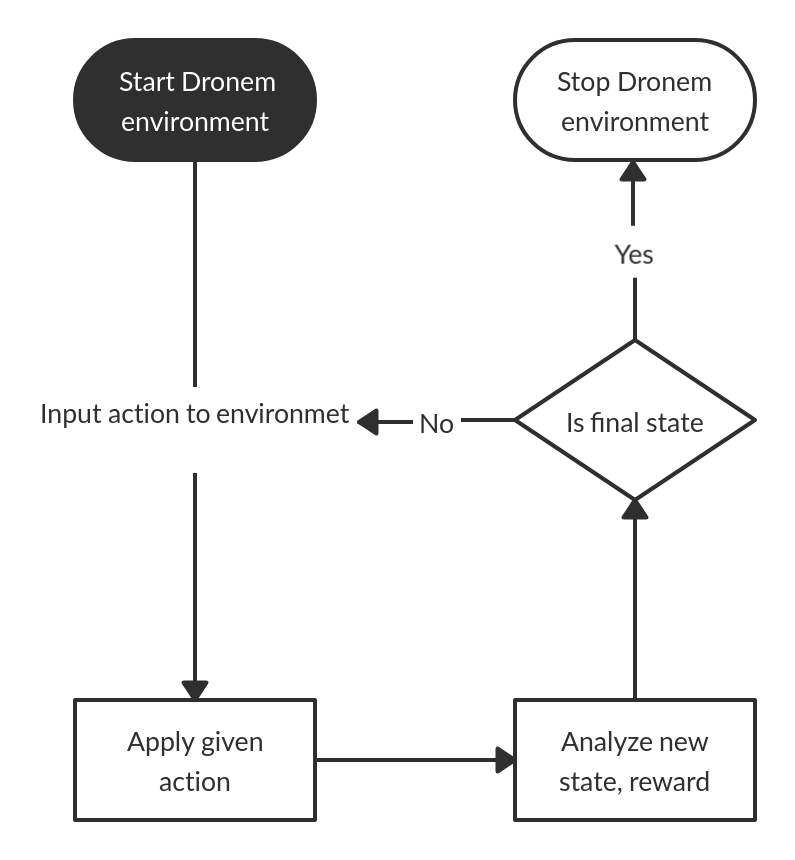
\includegraphics[scale=0.3]{Figures/Gym_env_flow.jpg}
    \caption{Dronem environment life cycle}
    \label{fig:dronemEnvPipeline}
\end{figure}{}

\begin{figure}[!htb]
    \centering
    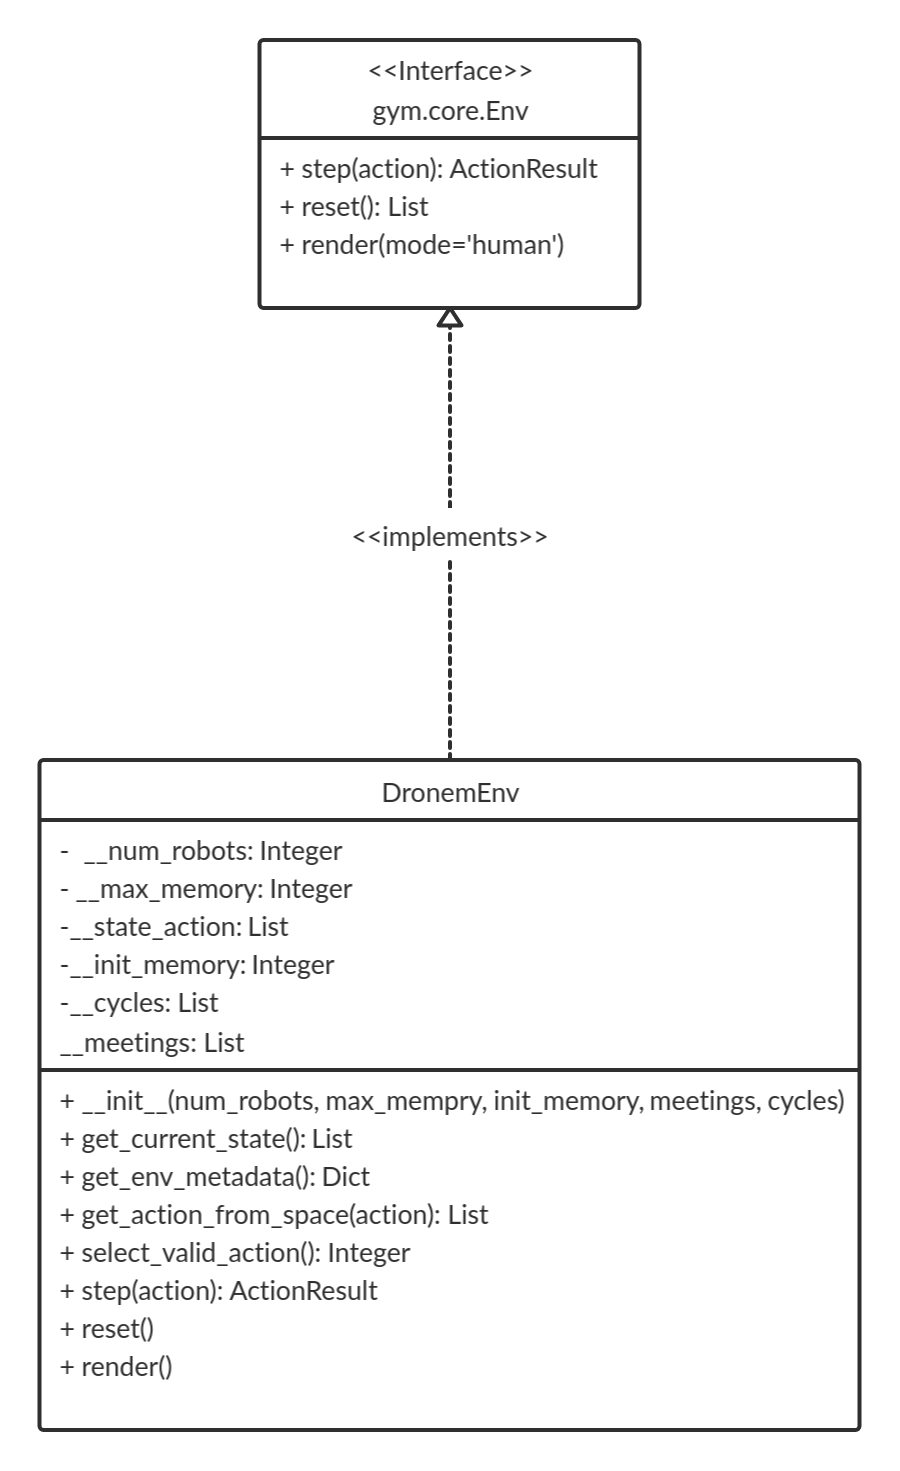
\includegraphics[scale=0.2]{Figures/gymEnvArchitecture.jpg}
    \caption{Dronem environment Gym architecture}
    \label{fig:dronemEnvGym}
\end{figure}{}


\subsection{Advantages and Disadvantages}

In the past, one of the problems in the reinforcement learning community was the lack of benchmarking tools, often the researchers were forced to code their own environments, and because no common interface was used, it was very hard for a research team to apply a reinforcement learning algorithm on environments created by others. 
\par This problem was solved by OpenAI Gym by not only exposing a common interface between all reinforcement learning environments, but also by offering more interesting environments as benchmarks such as the Atari Games. Even more, Gym offers a standardized test bed for algorithms in academic publishing.
\par The only inconvenience exposed by OpenAI Gym is the fact that only episodic reinforcement learning environments can be used, therefore for some environments a series of constraints have to be applied, while in the same time some RL classes of algorithms may not be suitable for episodic environments.

\section{Implementation}\label{implementation}
The implementation phase plays a major role in the life cycle of a software application, because big decisions are made in important aspects such as testing methodologies and development technologies. We will focus more on implementation aspects along this section.

\subsection{Backend}\label{BE}
Backend refers to any part of a software which is not accessible by the user and it is usually composed of a server which, together with an application acts as an operation manager and a database for storing application data. Backend technologies consist of a programming language, in our case \emph{Python}, and usually the programming language which is going to be used for development is enhanced by various frameworks such as \emph{Django}.

\subsection{Django vs Flask}

In recent years many web development frameworks for Python have been released, but none of them are nearly as popular as Django \cite{django} and Flask \cite{flask}. 
Django is an well-established framework having a bigger community of active users as it can be seen in Figure \ref{fig:DjangovsFlask}\cite{flaskvsdjango}, while Flask is a lightweight web framework.

\begin{figure}[!htb]
    \centering
    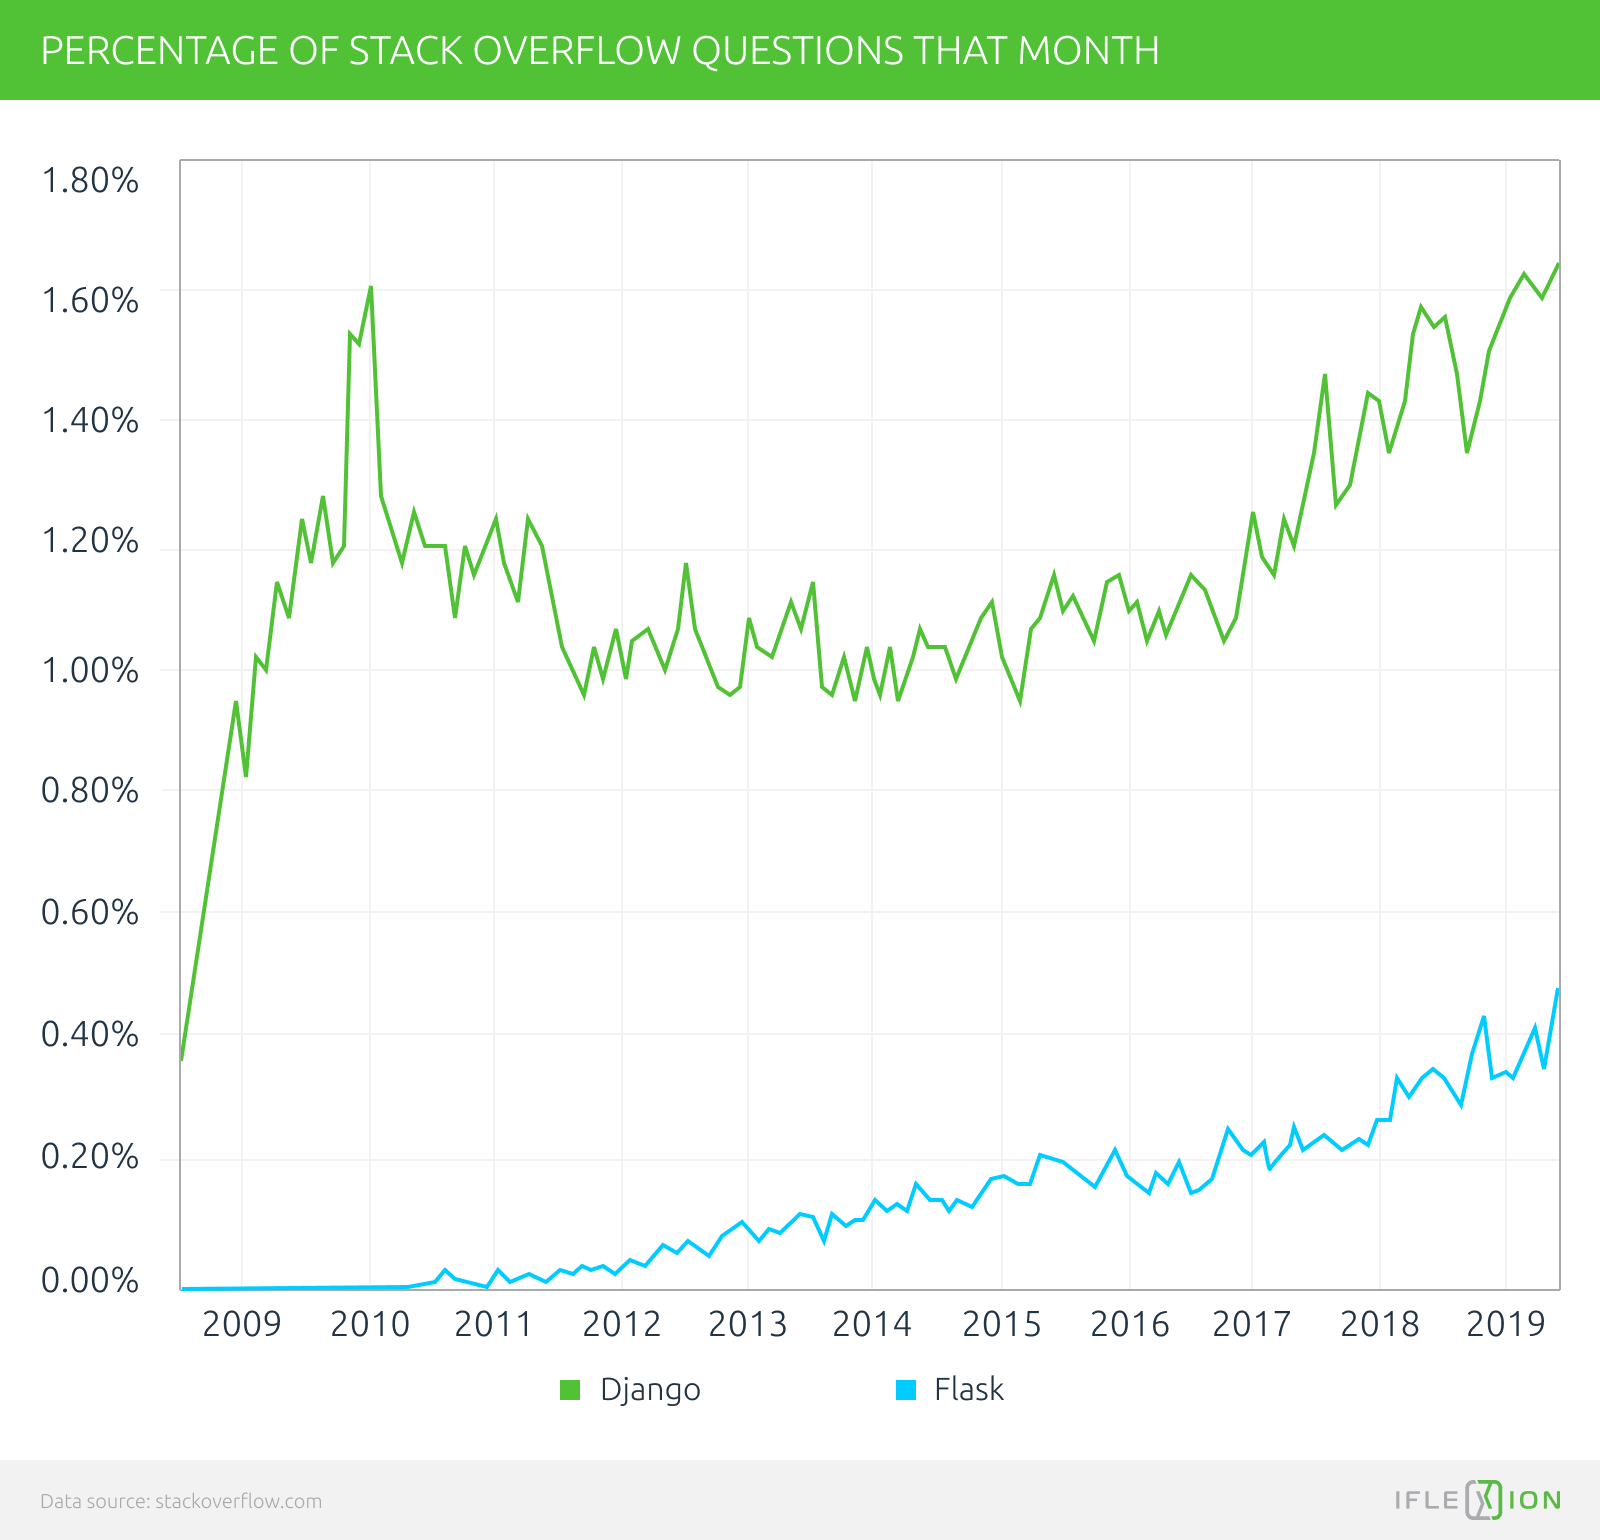
\includegraphics[scale=0.2]{Figures/djangovsFlask.png}
    \caption{Number of StackOverflow questions for Django and Flask}
    \label{fig:DjangovsFlask}
\end{figure}{}


\par Unlike Flask, Django has a 'battery included' philosophy, meaning that all you need in order to fully develop a web application is already included in the framework. Django makes it easier to handle common project administration tasks, by providing a fully functional admin interface, in order for the same functionality to be achieved using Flask, more packages needs to be installed and configured. Another advantage of Dajngo over Flask is allowing the developers to take advantage of a robust object-relational mapping (ORM) mechanism. The developers can use the ORM provided by Django to work with many popular databases such as MySQL, Oracle, SQLite, PostgresSQL whereas in Flask there is no ORM system built in. Flask requires developers to work with databases and perform database operations through SQLAlchemy \cite{sqlalchemy}.
\par Another argument which favors Django over Flask is the fact that developers can divide an application into multiple subapplications, hence it become easier for the developers to integrate new features into the application by splitting work and even reuse subapplications in other projects. Flask requires developers to create each project as a single application, however there is the option do add multiple models and views to the same application. When it comes to testing, both Django and Flask can use the Python integrated unittest framework, and both can be configured to use a secondary solution as necessary. However, the Django's integrated automated testing feature is a strong argument in its favor, especially when there is a need to create tests using dummy databases, as in Flask such a configuration is not trivial to accomplish.
\par As a conclusion, in order to build the Dronem Web application Django is the chosen framework because it offers many ways of creating scalable web applications through its ease of use, robustness, testing versatility and very active community.

\subsection{Django REST Framework}
While Django alone is sufficient in order to develop a scalable web application, in order to enhance it with the latest capabilities of manipulating and serializing data, Django REST Framework (DRF) will be used.
\par Django REST Framework \cite{drf} is a very powerfol toolkit for building Web Application Programming Interfaces (APIs). One of the biggest reasons to use DRF is that it makes it very easy to serialize data. The Django ORM is already a powerful tool for handling database migrations and queries, but it is not that easy to convert entities stored in the database to more used formats such as JavaScript Object Notation (JSON). This is the problem that DRF solves, by easing the conversion of objects stored in the database in formats such as JSON with just a few lines of code.

\subsection{Database}
These days, there is a big debate regarding the database type you should use for your project. Depending on what kind of data your application manages, there are SQL databases and NoSQL databases. For choosing what type of database is suitable for an application, the question "Is the data relational or not?" must be answered. Because our data is highly relational, we chose to use MySQL \cite{MySQL} as database, the following database schema is proposed for the Dronem Web application in Figure \ref{fig:dataBaseSchema}.


\begin{figure}[!htb]
    \centering
    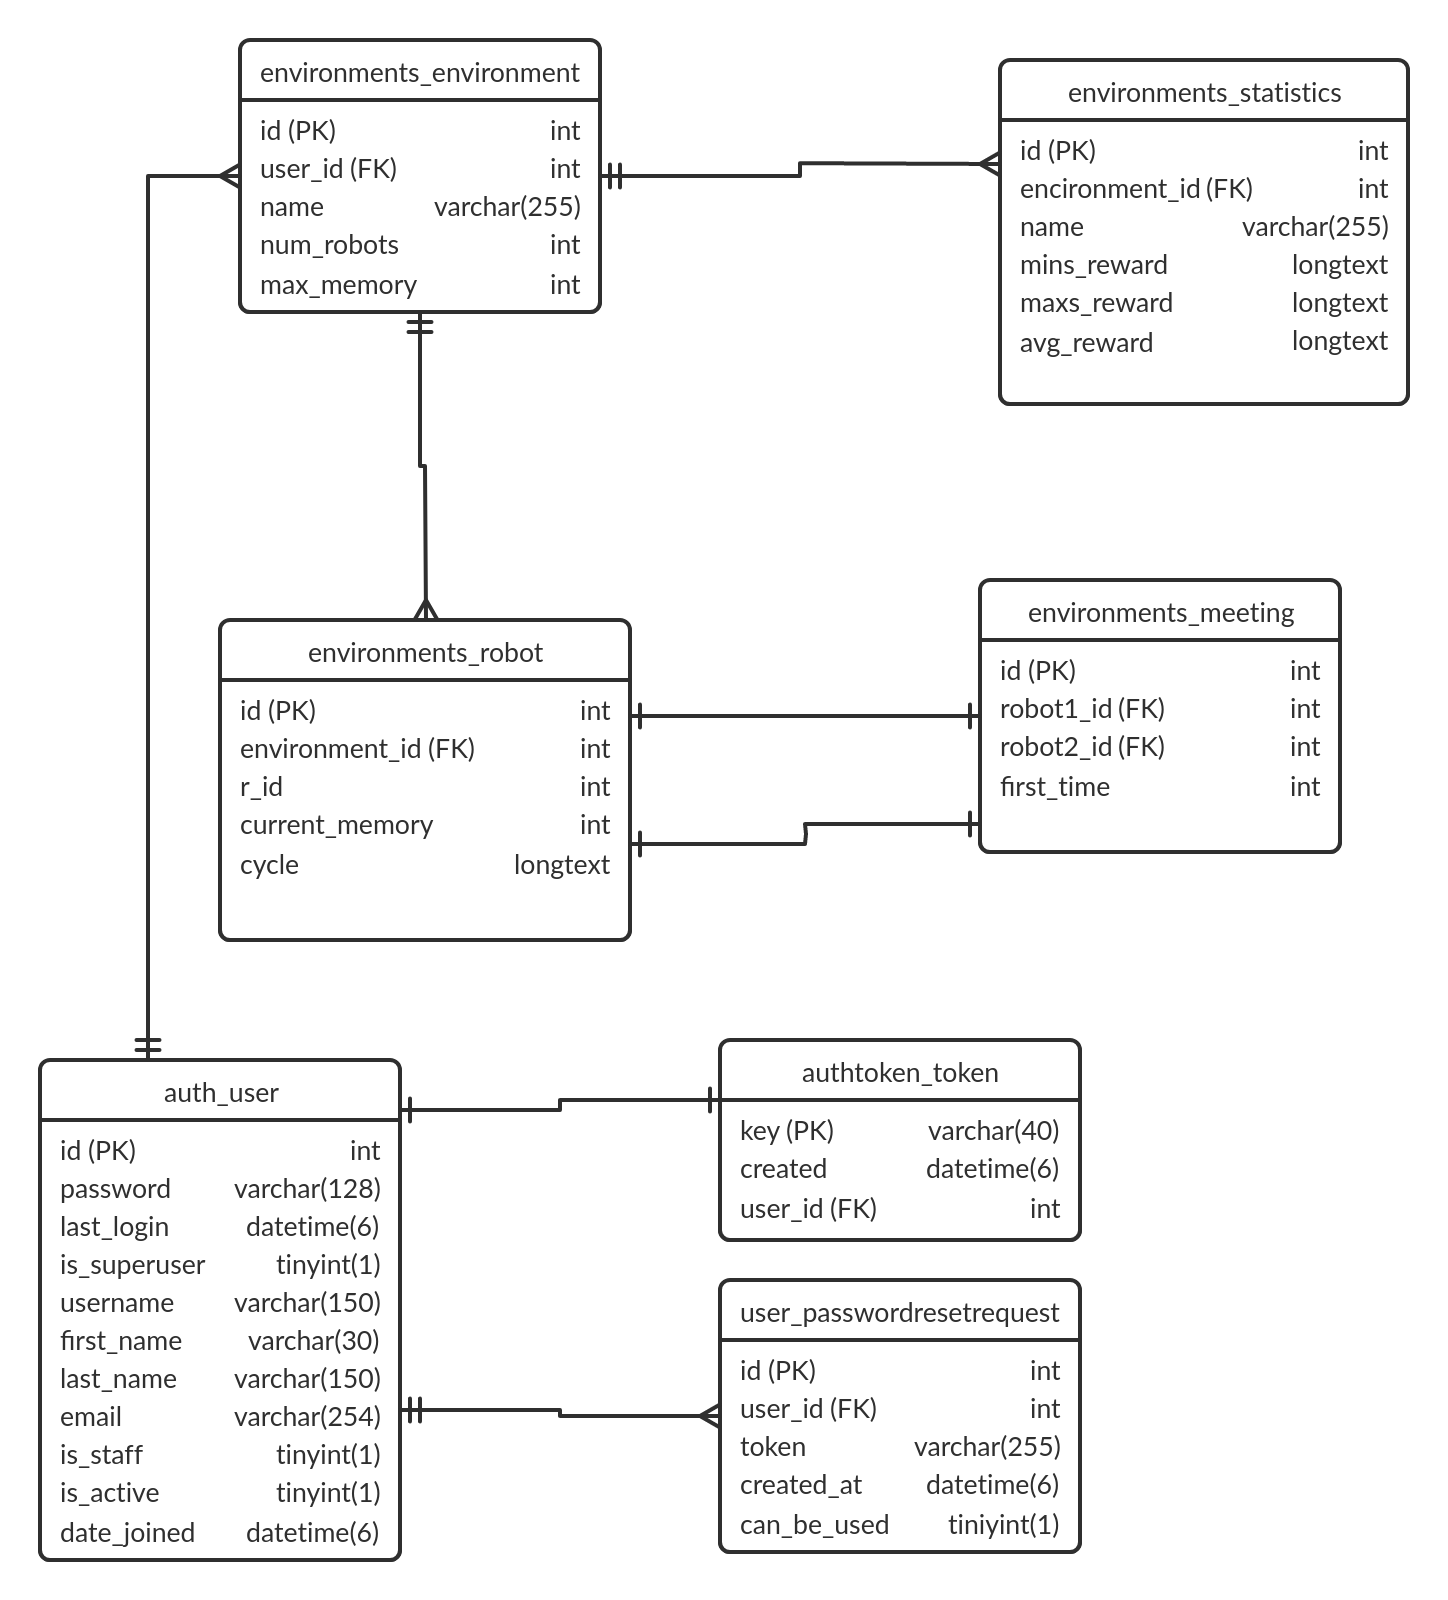
\includegraphics[scale=0.2]{Figures/databaseDiagram.jpg}
    \caption{Dronem Web database schema}
    \label{fig:dataBaseSchema}
\end{figure}{}

\subsection{Frontend}\label{FE}
As opposed to backend, the frontend side of a web application is concerned with the parts of the application which the user can see. The main tools used in frontend development are:
\begin{itemize}
    \item Hyper Text Markup Language (HTML) which is the backbone of any website. Being a markup language it means that it indicates that text can be turned into images, tables or other representations.
    \item Cascading Style Sheets (CSS) which controls the presentation aspect of the site.
    \item JavaScript which is an event-based imperative programming language used to add dynamic interactions to a website, while also maintaining communication with the backend side of the application.
\end{itemize}
\par The JavaScript language which is the most used programming language for frontend side applications, is usually enhanced using various frameworks and libraries such as the one used for the \emph{Dronem Web} frontend ReactJS \cite{react}. We chose ReactJS as our frontend library for JavaScript because it is proven to be highly scalable and extensible by maintaining several big web applications such as Facebook, Dropbox or Tesla.
\subsection{Design choices}

\subsubsection{REST vs GrapQL}
REpresentational State Transfer (REST) \cite{rest} is the most popular web architectural style providing a standard way of communication between computers on the web. Systems which use REST communication are often called RESTful. In order for an interface to be called RESTful the following requirements need to be meet:
\begin{itemize}
    \item Separation between client and server - the interface must separate the concerns of the client (frontend) and server (backend), by doing this the same interface may be used across multiple platforms and the server is more scalable by simplifying its components.
    \item Stateless - requests coming from the client must contain all the information needed in order to fulfill that request, and cannot be directly based on previous requests. 
    \item Cacheable - every response needs to be labeled as being cacheable or not as the client can use that response for future equivalent requests.
    \item Uniform interface - Applying software engineering guidelines, having an uniform interface, the overal complexity of the system is minimized.
    \item Layered system - The architecture of the system must be composed as an hierarchical structure.
\end{itemize}

\par GraphQL\cite{graphQL} on the other hand is a query language for an API and a server-side runtime for executing queries by using a type system defined for the application data. It was created by Facebook and it is supposed to fundamentally change the way applications communicate  across the web. GraphQL promises to solve the main problems which arise from using REST, such as over and under data fetching. Over-fetching means downloading unnecessary data, which is a common problem encountered when using REST, because a REST endpoint can only return fixed data structures. Returning fixed data structures also causes under-fetching, for example think about making a call to retrieve a list of users, then for every user we have to make another request to retrieve their followers. This problems are solved by GraphQL with an ingenious solution, declaring specific queries, which give no more, no less, but the necessary data. 

\par Because GraphQL is still an emerging technology, we chose to use REST for the Dronem Web application, but as more and more documentation and applications using GraphQL will start to appear, we will consider enhancing our application by replacing the RESTful interface with GrapQL.

\subsubsection{Redis}

Redis (REmote DIcrionary Server) \cite{redis} is an open source in-memory data-structure, used as a database, message broker and cache. At a high level Redis can be viewed as key-value database, each value is mapped by a key.
It supports various types of data structures such as strings, hashes, sets, lists, sorted sets etc. Values can only be retrieve it its key is known.
Once installed in a server Redis is very easy to operate using Redis Command Line Interface (CLI), having the following main features:

\begin{itemize}
    \item Speed - Redis is capable of loading a whole dataset in memory, approximately 81.000 GETs/second.
    \item Many Supported Languages - There are many programming languages which support Redis bindings by default.
    \item Master/Slave Replication - Redis supports a very simple and fast Master/Slave replication, being so simple that in only needs one line of configuration.
\end{itemize}

The main reason Redis has been chosen to be the message broker for the Dronem Web application is that it has a different evolution path in the key-value databases where values can store more complex data types such as our training configurations for environments, with atomic operations on those complex data types.

\subsubsection{Celery}
Celery \cite{celery} is a task queue (mechanism to distribute work across machines) used in Django. Its main use cases are:
\begin{itemize}
    \item Tasks that need to run asynchronously.
    \item Heavy background computations.
    \item Periodic tasks.
    \item Interaction with external API's.
\end{itemize}

\par Celery communicates via messages, using a broker such as Redis or RabbitMQ, whose goal is to mediate between clients and workers. In order for the client to initiate a task, the client adds a messages into the queue, then the broker assigns the message to a worker. After the worker finishes its job the effects of the task are stored in a task store result, in our case the database.

\par Because training an environment is not an instantaneous task we want to exclude the process from the request-response HTTP cycle. In order to achieve this, whenever a user requests an environment training a Celery task is started so that a user can train multiple environments in the same time while also being able to use other features of the application because it is not limited by the request-response HTTP cycle (i.e. the user does not need to wait until the training process is complete in order to use the application).

\subsection{Testing}
Following the software development methodology stated in Section \ref{softDev}, one of the most important activities is testing, as most of the time software testing determines the quality of software after a programmer develops it. The testing process involves evaluating information that is related to a product. Also testing ensures that the application satisfies the security requirements in order to protect confidential data.
\par While there are many software testing techniques and procedures we choose to use testing based on specification (Black Box Testing) and testing based on implementation (White Box Testing). Combining the two mentioned techniques in practice yields the best results, by using the Equivalence Class Partitioning (ECP) and Boundary Value Analysis (BVA) from Black Box Testing and Cyclomatic Complexity (CC) and the coverage criteria from White Box Testing.
\par In order to create flexible and easy to write tests the Pytest\cite{pytest} framework was used. Pytest is a framework which allows to write Python tests for different application levels including database, API or User Interface (UI). One of the most important advantages of Pytest over other testing frameworks is the ease of use and test readability, which are key features when it comes to testing.
What differentiate Pytest from other testing frameworks is the usage of a system based on fixtures (functions which initialize test functions), instead of using the classic \emph{setUp}, \emph{tearDown} testing system.
Another important feature of Pytest is the ease of creating \emph{mock} objects using a special fixture, called \emph{monkeypatch}, which allows changing the behaviour of any Python object with only one line of code.

\par For the Dronem Web application, several tests were designed and implemented in order to ensure that the application works according to the system requirements defined in Section \ref{ad}. Extensive testing was done around the \emph{QLearning} algorithm and the \emph{DronemGymEnv} architecture, while numerous tests were conducted for the API of the application in order to ensure optimal functionality.
\subsection{Documentation}
Documenting application is a mandatory activity in software development because good documentation makes it easier for the developers to maintain and add new features to the application. The main focuses of a documentation are development, maintenance and knowledge transfer to other developers. Usually the principal components of a documentation concern with server environments, databases, troubleshooting, application installation and code deployment.
\par The documentation for the \emph{Dronem Web} application is composed of two main parts. The first part consists in detailed comments for every relevant function, including input parameters, requirements and effects. Also detailed comment blocks were written for the \emph{DronemGymEnv} environment highlighting the main characteristics of the environment. The second part of the documentation is represented by the API documentation which was automatically generated using Django REST Swagger. An example of the API documentation generated for one REST \emph{/users/signin/} path can be saw in Figure \ref{fig:apiDoc} 

\begin{figure}[!htb]
    \centering
    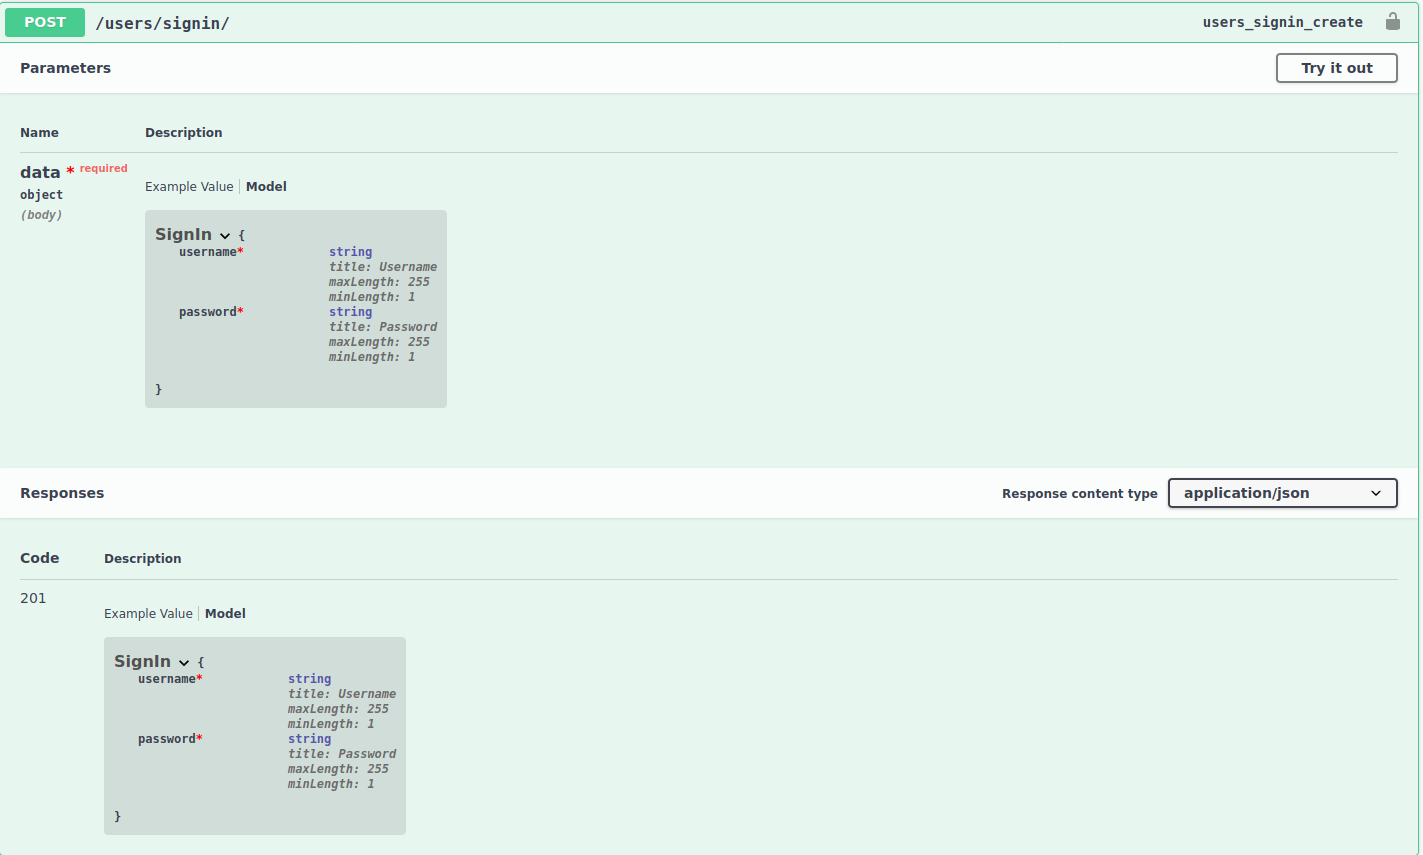
\includegraphics[scale=0.3]{Figures/apiDoc.png}
    \caption{API documentation for \emph{/users/signin/} path}
    \label{fig:apiDoc}
\end{figure}{}

\section{User manual}\label{userManual}
It is very important to write a good User Manual of the application in order to ease the first interactions of the user with the main functionalities of the platform, hence this section is focused on familiarizing the user with the application.

\subsection{Creating environments}
To achieve creation of an environment the user must click the Add Environment tab in order to to have access to the environment add form shown in Figure \ref{fig:addEnv}.
After that, the user can choose between adding the environment through a JSON file or by completing the multi-step form, of course the preferred way is via a JSON file, as adding a big environment by hand using a form is a tedious work. After completing the multi step form, or uploading the JSON file, an \emph{Add Environment} button will appear, clicking it will result in creating a new environment.


\begin{figure}[!htb]
    \centering
    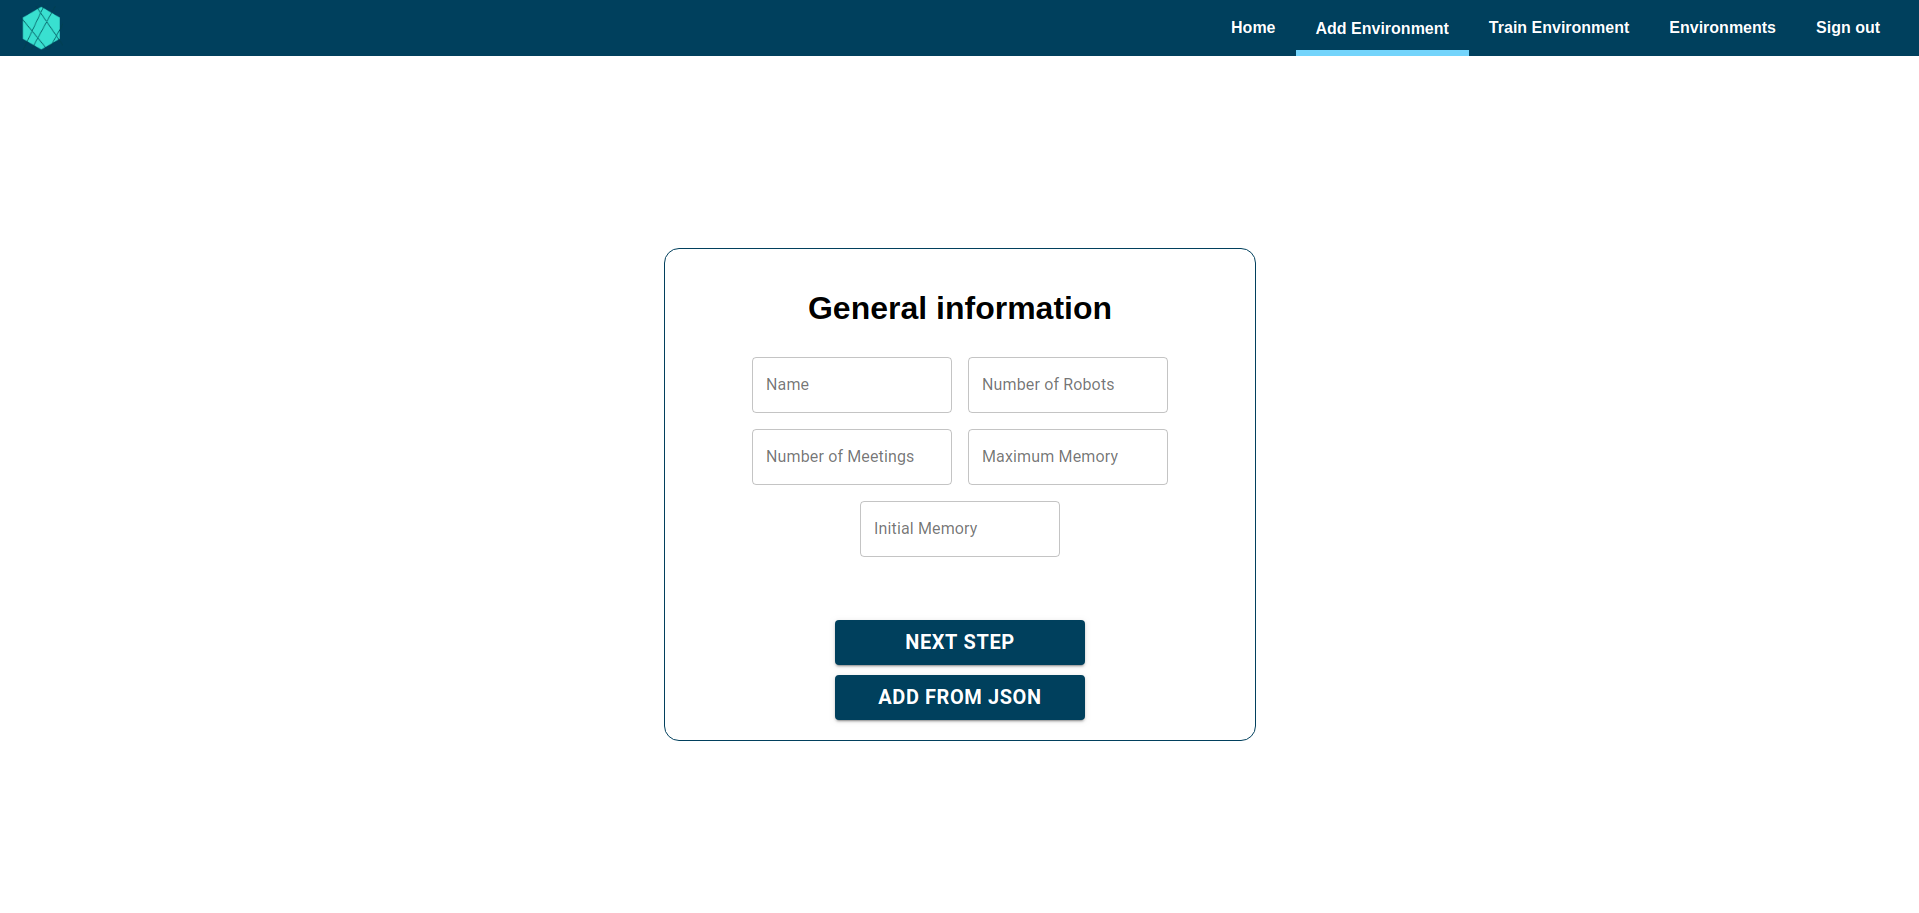
\includegraphics[scale=0.22]{Figures/addEnvsView.png}
    \caption{Drone Web add environment view}
    \label{fig:addEnv}
\end{figure}

\subsection{Training environments and downloading Q-tables}
\subsubsection{Training an environment}
In order to start a training session, the user must select the \emph{Training Environment} tab. After clicking the training tab, the screen shown in Figure \ref{fig:trainView} will appear, the user must select an environment and input the training parameters for the algorithm. Finally clicking the Train button will start a training session, and live statistics of the training will appear on the canvas situated on the right side of the screen.

\begin{figure}[!htb]
    \centering
    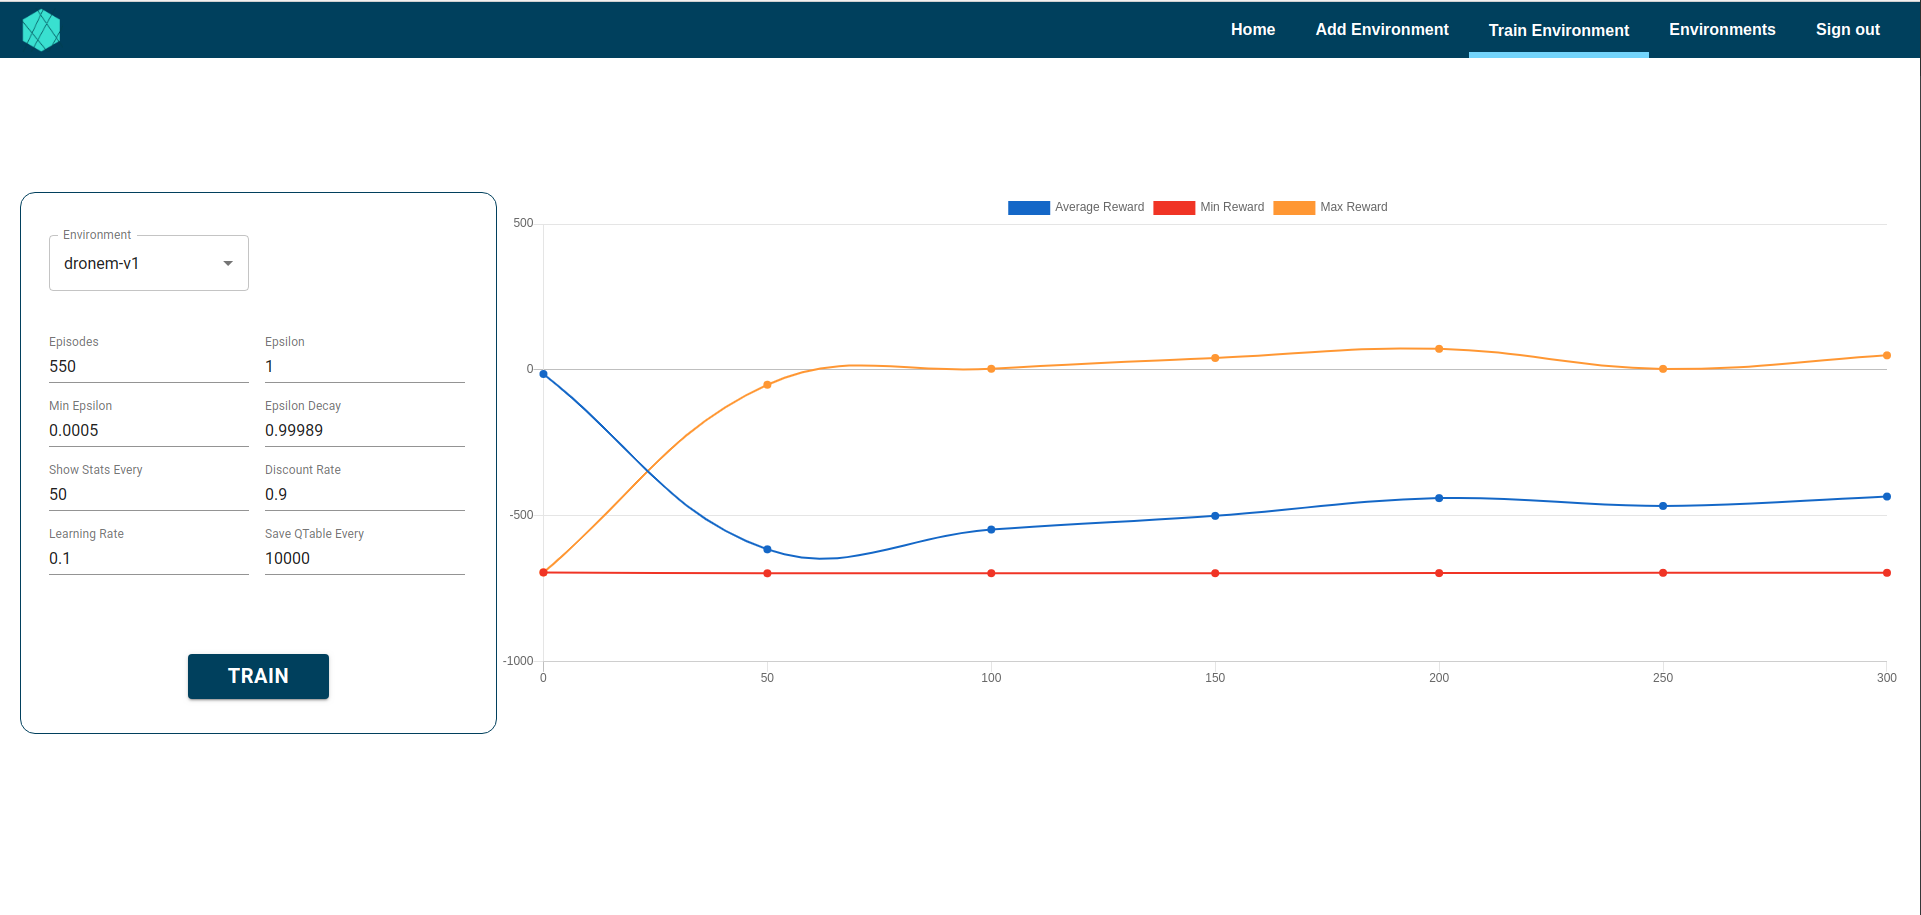
\includegraphics[scale=0.22]{Figures/trainView.png}
    \caption{Drone Web train view}
    \label{fig:trainView}
\end{figure}


\subsubsection{Downloading Q-tables}
The environments tab, presents numerous functionalities as can be observed in Figure \ref{fig:ensvView}. The user can download a JSON file containing the best Q-table for an environment by clicking the \emph{Download Best QTable} button. 

\begin{figure}[!htb]
    \centering
    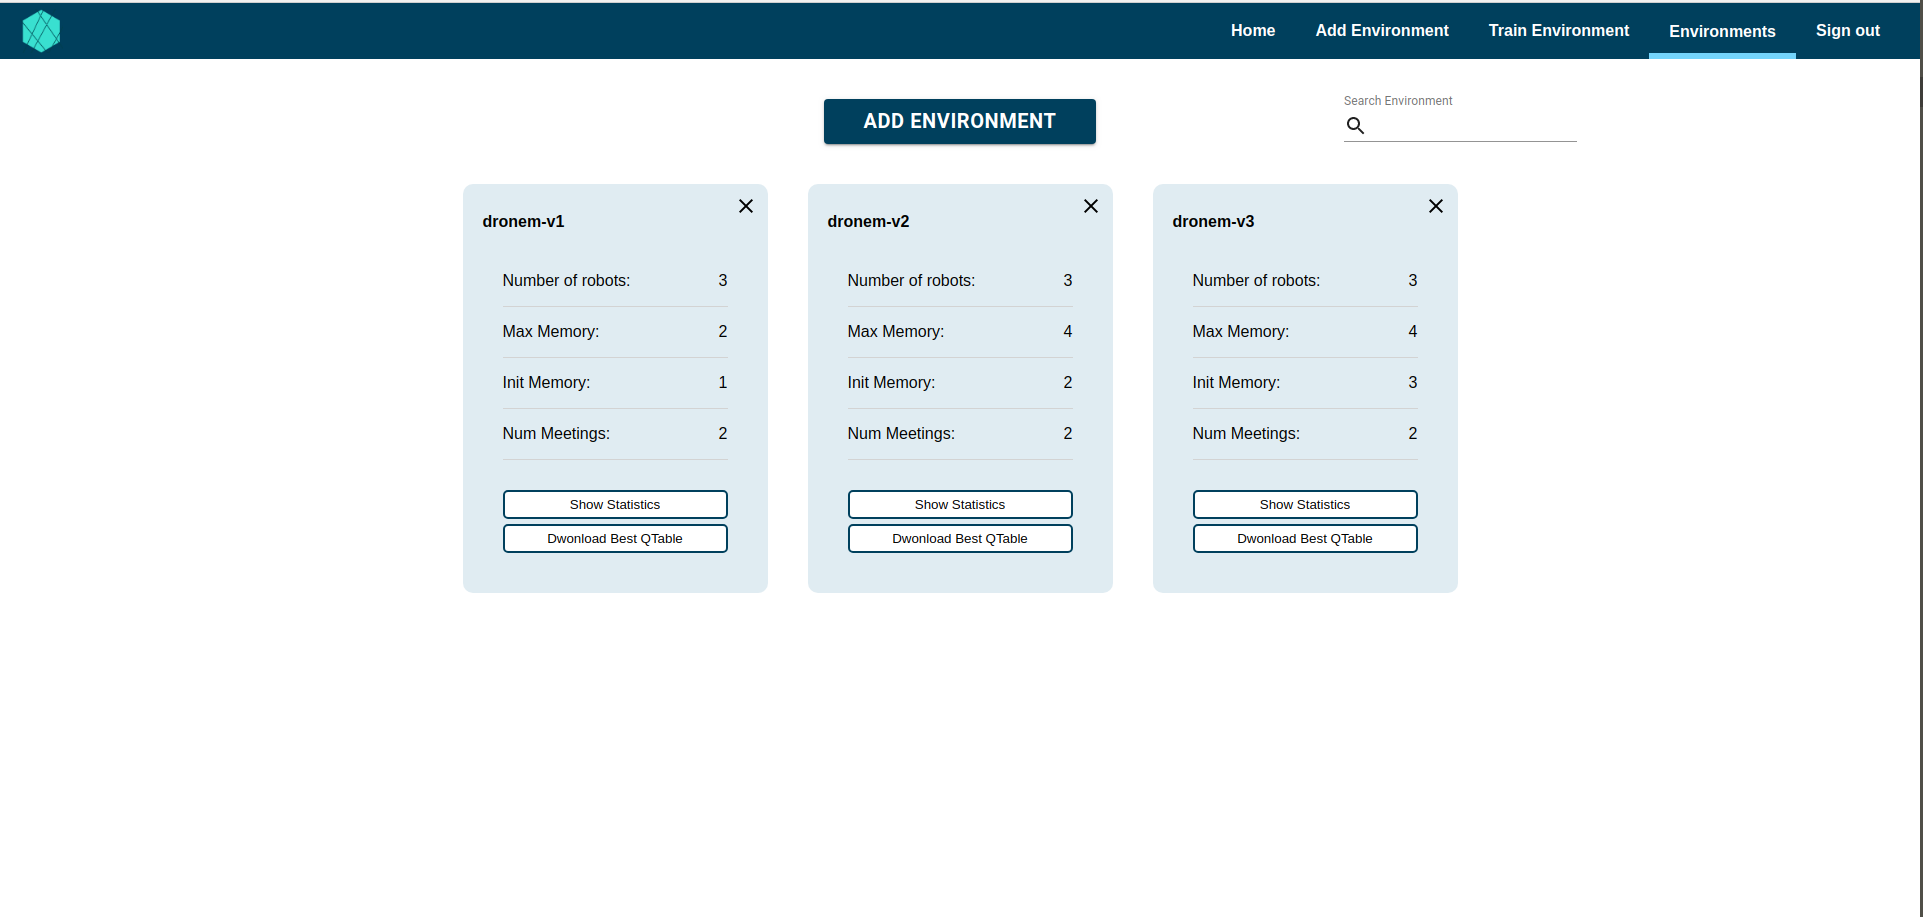
\includegraphics[scale=0.22]{Figures/environmentsView.png}
    \caption{Drone Web environments view}
    \label{fig:ensvView}
\end{figure}

\subsubsection{Showing training statistics}
Also the user can retrieve statistics about past training of an environment, by clicking the \emph{Show Statistics} button, leading to the view depicted in Figure \ref{fig:statisticsView}


\begin{figure}[!htb]
    \centering
    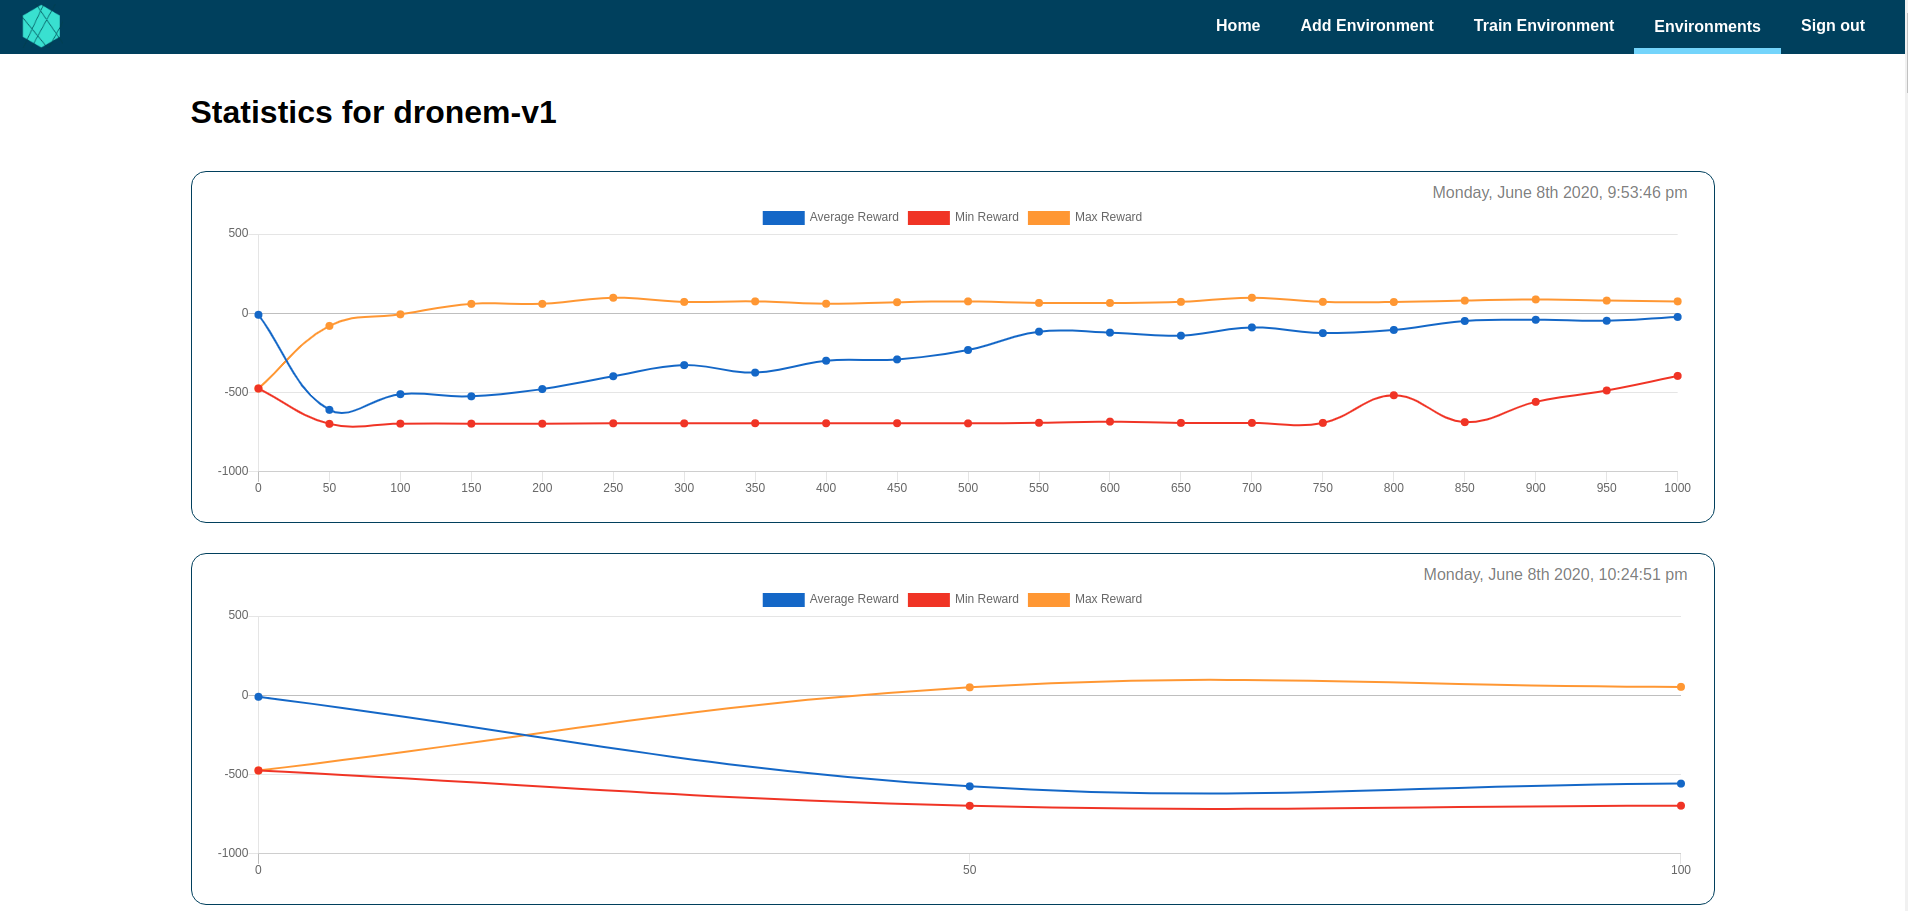
\includegraphics[scale=0.22]{Figures/statisticsView.png}
    \caption{Drone Web statistics view}
    \label{fig:statisticsView}
\end{figure}


\section{Discussion}\label{softDiscussionn}
The purpose of this chapter was to present the software development process followed in order to develop the \emph{Dronem Web} application. Several development activities were documented along this chapter, starting with analysis and design, implementation, testing and documentation of the application while outlining the importance of following a software development methodology when constructing an application and what catastrophic consequences can arise when no strategy is used. This section presents the original contributions and benefits brought to the Reinforcement Learning community by the creation of this application.

\par First of all the \emph{Dronem Web} is, to the best of our knowledge, the only application available for creating, manipulating and training MRP environments. We presumably think that more and more users will start using our application for different tasks ranging from university level projects to real world problems such as smart surveillance systems, as long as there is a suitable MRP modelling for those problems. Another original contribution of our application consists in the possibility to retrieve the Q-table for the best training session of an environment, hence the training results can be further used in real applications that are modelled as MRP problems. Also we encourage the users to further extend our \emph{Dronem Gym Environment} which will be publicly available at: \url{https://github.com/GeorgianBadita/Dronem-gym-envirnoment}. We hope to grow a flourishing community of RL enthusiasts around our application who will further develop the foundation presented by this thesis.

\par Being constructed with the latest technologies and with the best software development practices, we believe the Dronem Web application to be very scalable, being able to handle many users and training sessions in parallel if deployed on capable enough hardware.

\section{Future enhancements}\label{futureEnh}
 This application is laid as a foundation for an efficient way to create, manipulate and train MRP environments, but it opens up several paths for future enhancements.

\par As every application strives to be better and better, we think that our application may benefit from  some enhancements too. First of all, the application is limited in the types of environments it can manage, users are able to only create and train environments corresponding to the specification defined in Chapter \ref{flow}. In the future we are going to add the possibility to manipulate different types of environments or even create environments for different reinforcement learning problems.

\par When it comes to training times, currently for some environments waiting times are very high, due to the fact that the application runs on a computer with low system specifications. A possible solution to overcome this issue would be to deploy the backend of the application on a much more powerful machine, reducing training times significantly, for example an EC2 Amazon Web Services (AWS) instance can be used. A task framework solution has already been implemented in order to reduce training times, but as python is not a 'real' multithreaded programming language, because of its Global Interpreter Lock (GIL), other solutions need to be taken into consideration.

\par Another important area where the Dronem Web application can be improved is the crash recovery. If the machine where the backend of the application is stored crashes, or even if the Redis or Celery services stop working all environments which are trained in that moment will stop and every interaction with the application will fail. Hence, a mechanism for crash recovery is also needed to be considered for the application, so that after any service crash all training environments should return to their state before the crash. One solution for this problem would be to save the entire application state in the database whenever a training step is taken, although this would increase training times, it will ensure that the application can recover whenever a something bad happens. Nevertheless more research in this direction is needed and more enhancements will be taken into consideration in the future.

\chapter*{Conclusions}
\addcontentsline{toc}{chapter}{\textbf{Conclusions}}
\label{conclus}


This thesis investigaes the data delivery optimization problem in a simplified setting  of the \emph{multi-robot patrolling} problem, in which the environment is deterministic. Accordingly a centralized and offline approach $DynFloR$ based on flows in dynamic networks was introduced. The goal of $DynFloR$ is to determine the robots' policy for maximizing  the quantity of data delivered to a base station in a given time, assuming that the robots are continuously collecting data during their patrolling. The more general aim of the research initiated in this thesis is to prove that a \emph{reinforcement learning} approach of the MRP problem is highly feasible, and that further research conducted in this direction could lead to impressive results. Therefore, we introduced a reinforcement learning approach $DronemRL$, which is an improvement of the foundation laid by $DynFloR$.

More contributions have been made in this thesis by designing, implementing and documenting the \emph{Dronem Web} application, which to the best of my knowledge is the only application publicly available capable of modeling and training multi-robot patrolling environments. In order to create the application, a client-server architecture was designed;  the main libraries and frameworks used were:  OpenAI Gym, Django, Django Rest Framework, and ReactJS - ensuring a scalable architecture. I am confident that in the future, many reinforcement learning enthusiasts  will start using this application as a learning tool, because it is easy to use, intuitive and efficient. 

Further work will extend the experimental evaluation and theoretical analysis of $DronemRL$ in order to better assess its performance. I also aim to decentralize the decision making process and to incorporate uncertainty in the communication between robots. In order to achieve these goals, a very refined Deep Q-learning perspective might be considered. 



\bibliographystyle{alpha}
\bibliography{bib}

\end{document}